\section{Results and Discussion}\label{sec:results_and_discussion}

\subsection{Bathymetric domain and baseline sea-only routing}
\label{sec:results_bathy_baseline}

We first define a static bathymetric routing grid for the trans-Arctic corridor.
Bathymetry is taken from the GEBCO\_2024 global grid and subset to the region
$40$--$85^{\circ}$N and $20^{\circ}$W–$180^{\circ}$E, which captures the North
Atlantic, Barents and Kara seas, the Eurasian Arctic shelf and the Bering and
North Pacific gateway. The native GEBCO field (15~arcsec) is coarsened to a
regular $0.5^{\circ}\times0.5^{\circ}$ latitude--longitude grid yielding a routing grid of $89\times399$ nodes
(Fig.~\ref{fig:bathy_domain_components}a). Within this domain, depths on the
routing grid range from approximately $-8700$~m in the deep basins to $+5600$~m
over land.

A binary land/sea mask is constructed by classifying grid cells with
GEBCO elevation $\leq 0$~m as sea and $>0$~m as land
(Fig.~\ref{fig:bathy_domain_components}b). Connected-component labelling on the
sea mask shows that the largest sea component forms a continuous oceanic
corridor from the North Atlantic to the North Pacific across the Arctic, while
smaller components correspond to enclosed shelf seas and fjords. This mask
defines the static sea-only feasibility constraint used throughout the
remainder of the study.

To obtain a canonical baseline route, we consider an idealised
trans-Arctic origin–destination (OD) pair between a North Atlantic waypoint at
$(40.5^{\circ}\text{N},\,19.5^{\circ}\text{W})$ and a North Pacific waypoint at
$(69.5^{\circ}\text{N},\,179.5^{\circ}\text{E})$, corresponding to the
south-western and north-eastern corners of the routing domain. The great-circle
distance between these two waypoints is $4149.6$~NM. Routing on the $0.5^{\circ}$
grid is performed using an A* search with edge costs equal to the great-circle
distance between neighbouring grid nodes, restricted to cells in the static
sea mask. The resulting sea-only route is shown in
Fig.~\ref{fig:seaonly_route} and runs northwards out of the North Atlantic,
skirts the Eurasian Arctic shelf break and exits into the North Pacific.

The sea-only route distance is $4561.1$~NM, i.e.\ approximately $10\%$ longer
than the unconstrained great-circle distance. At a design speed of 14~kn this
corresponds to a travel time of 13.6~days, compared to 12.4~days for the
great-circle, implying a penalty of about 1.2~days purely due to enforcing
sea-only feasibility on a coarse grid. Bathymetry sampled along the route
(Fig.~\ref{fig:depth_profile}) indicates that the path remains predominantly in
deep water: depths along the route have a mean of $\approx -3300$~m, with a
minimum of $\approx -5700$~m and a shallowest segment of $\approx -30$~m. The
associated depth histogram shows that the route samples the deeper part of the
corridor-wide depth distribution, with only a few segments approaching the
continental shelf. This confirms that the purely geometric sea-only constraint
already tends to select deep-water pathways, even before any explicit
bathymetric safety threshold is applied.

\begin{figure}[htbp]
  \centering
  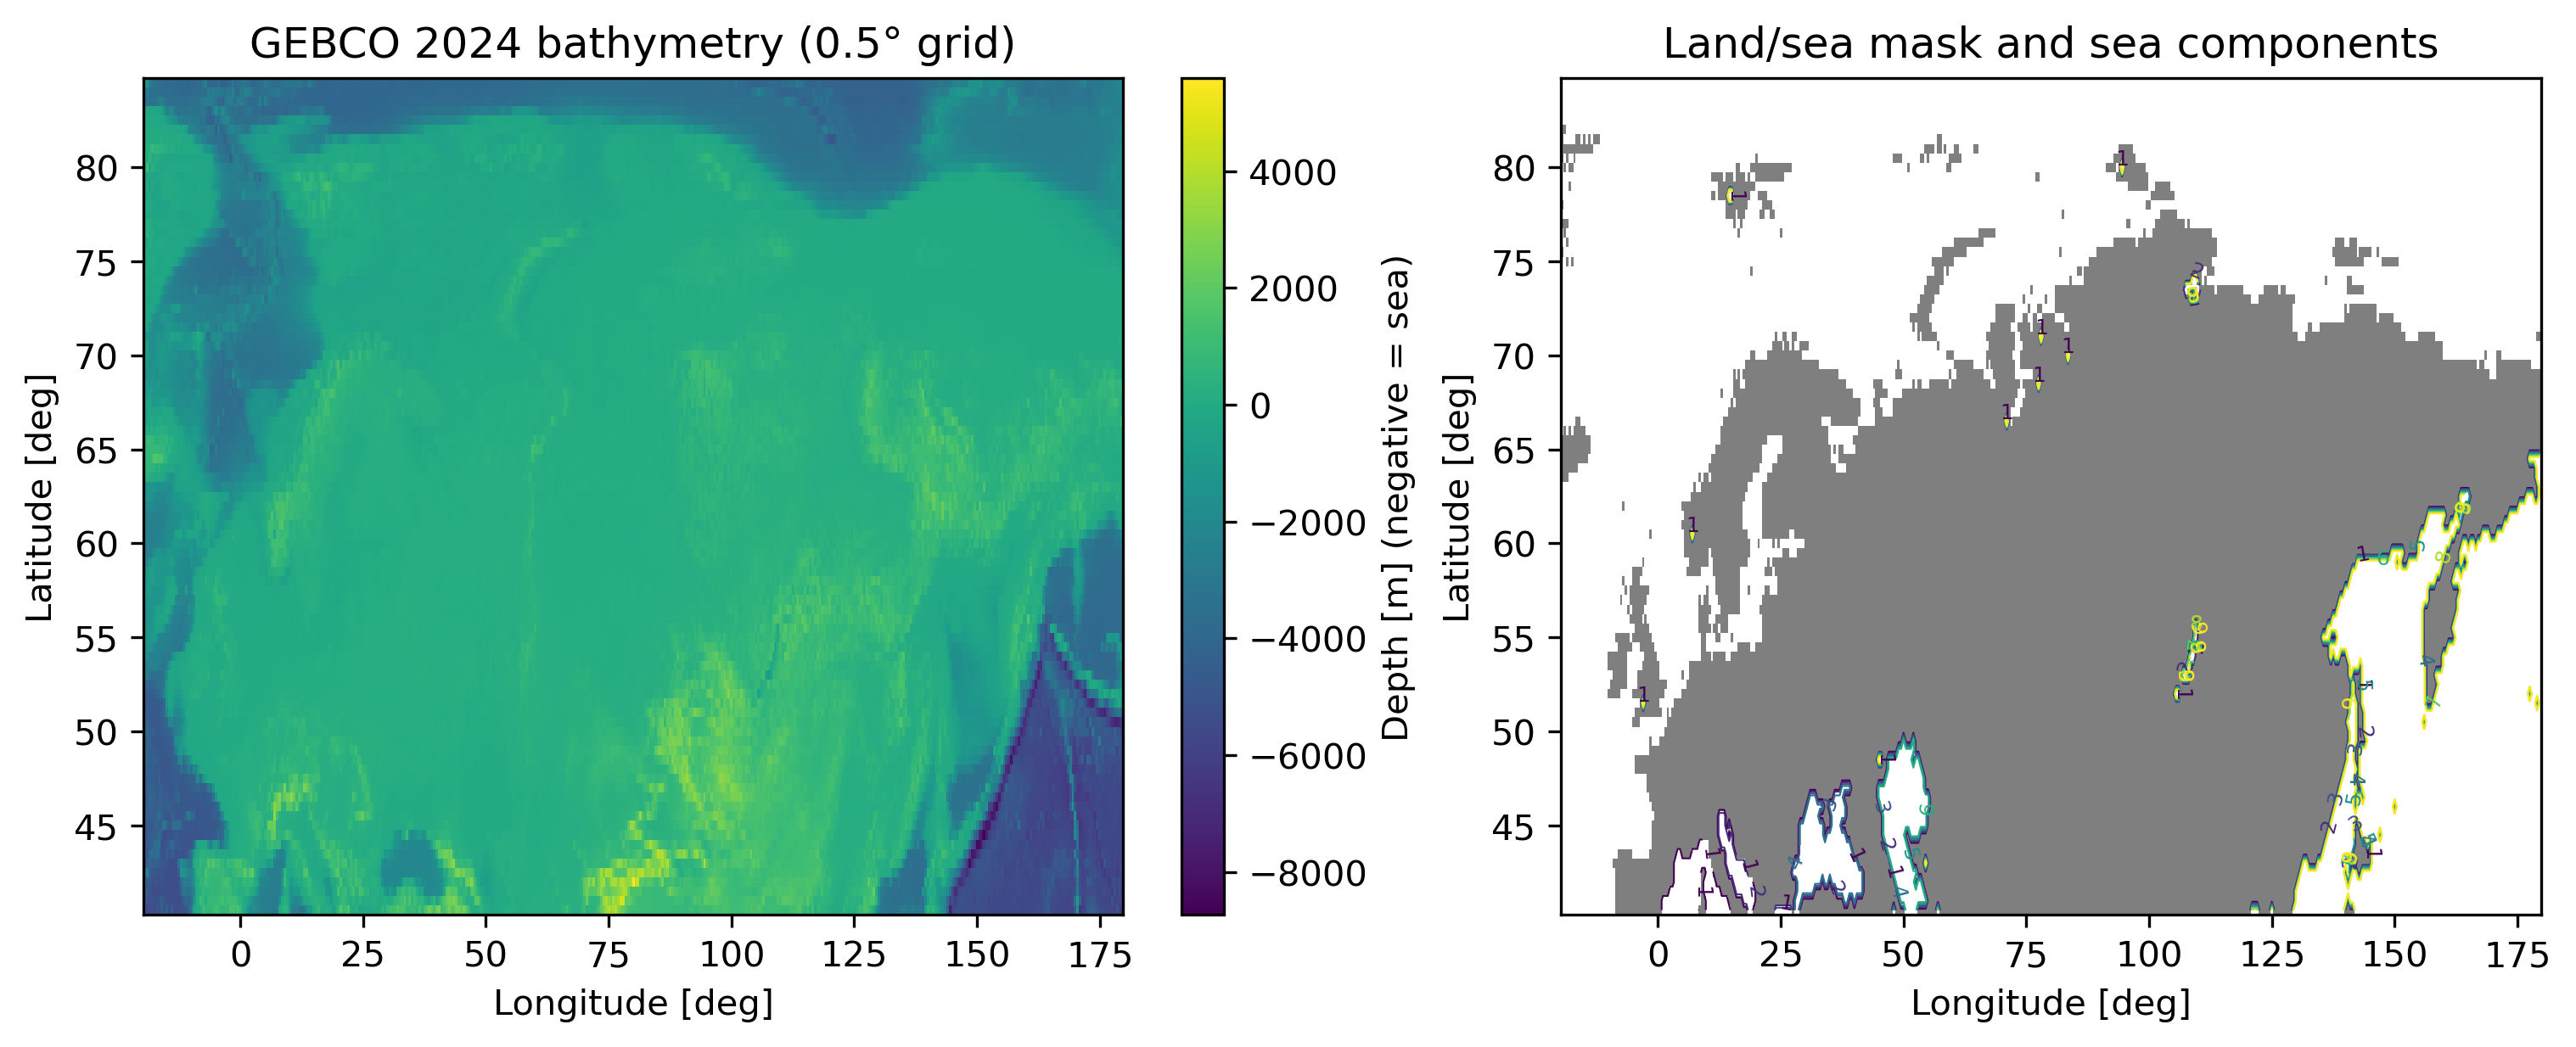
\includegraphics[width=\linewidth]{fig01_bathy_domain_mask}
  \caption{%
  (a) GEBCO~2024 bathymetry coarsened to a $0.5^{\circ}\times0.5^{\circ}$ routing
  grid over the Arctic corridor (40--85$^{\circ}$N, 20$^{\circ}$W–180$^{\circ}$E).
  (b) Derived land/sea mask and connected sea components; the largest sea
  component links the North Atlantic and North Pacific, while smaller ones are
  enclosed shelf seas and fjords.%
  }
  \label{fig:bathy_domain_components}
\end{figure}

\begin{figure}[htbp]
  \centering
  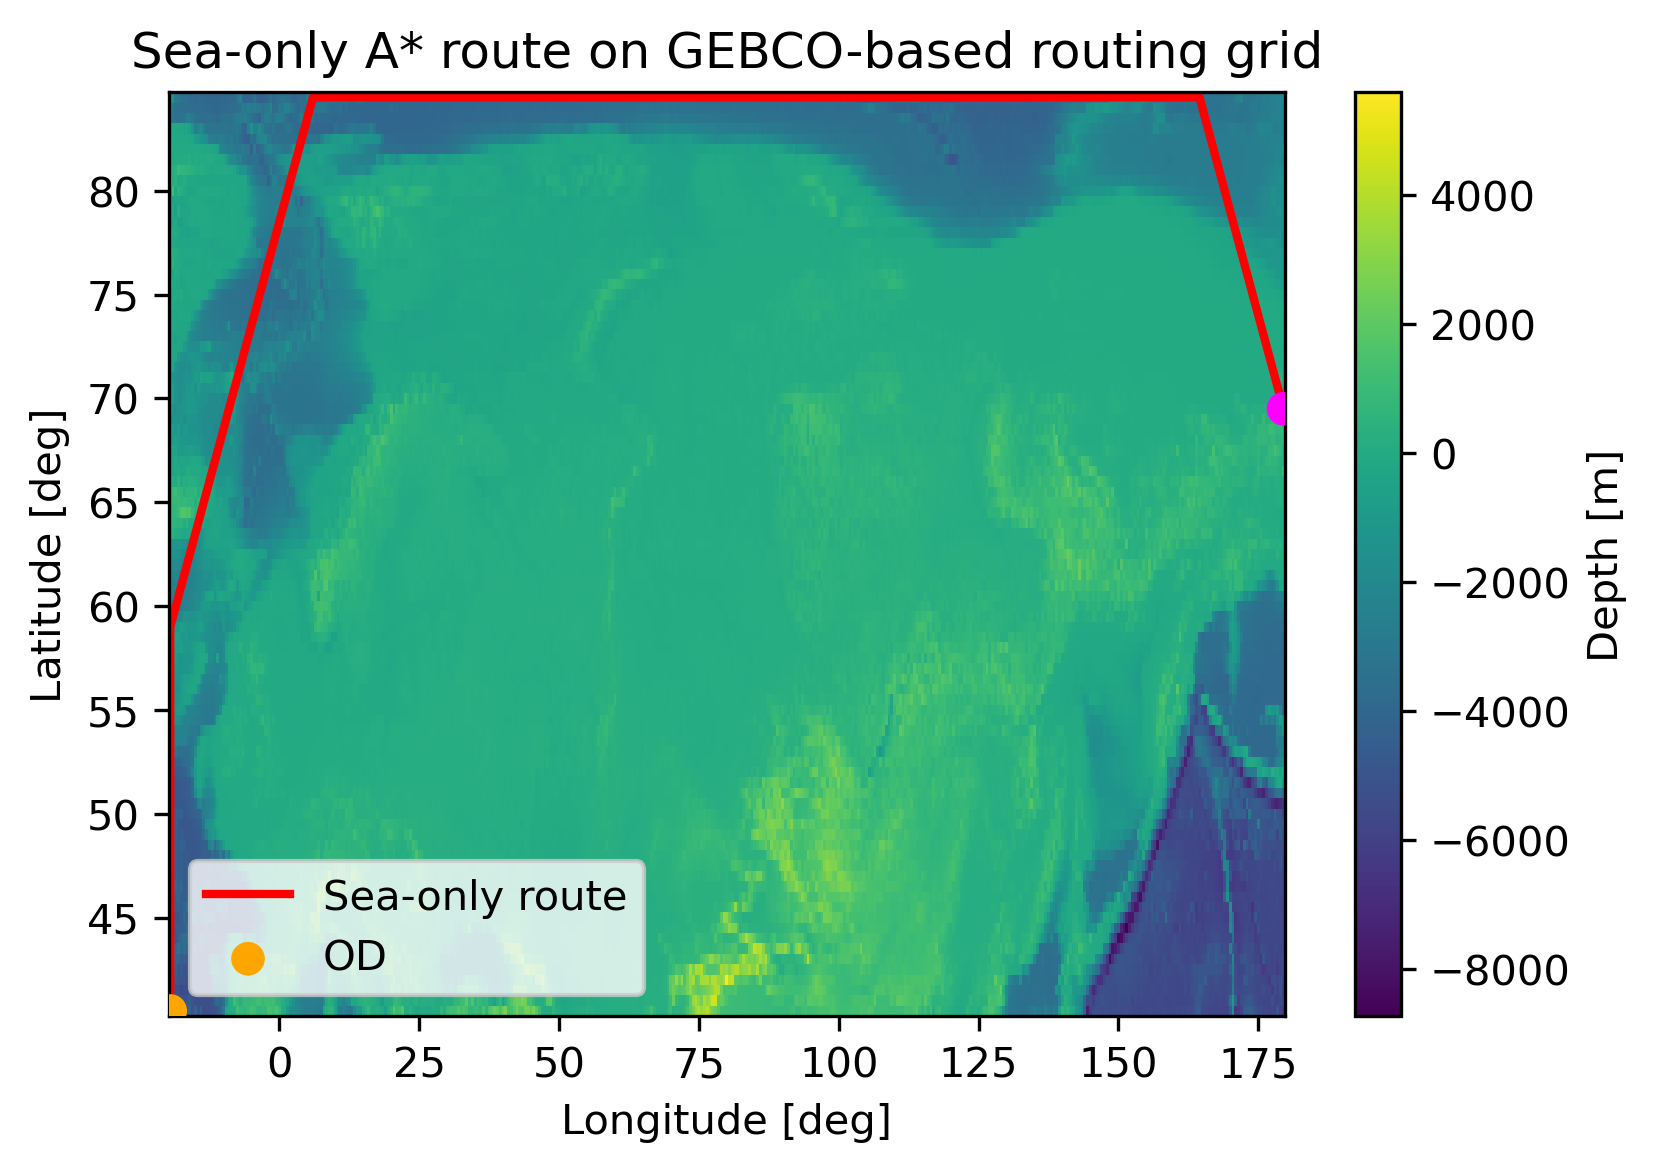
\includegraphics[width=0.75\linewidth]{fig02_seaonly_route}
  \caption{%
  Sea-only A* route (red) between the canonical origin--destination pair
  overlaid on the GEBCO-based $0.5^{\circ}$ bathymetry. The route remains within
  the static sea mask and follows deep-water pathways along the Arctic margin.%
  }
  \label{fig:seaonly_route}
\end{figure}

\begin{figure}[htbp]
  \centering
  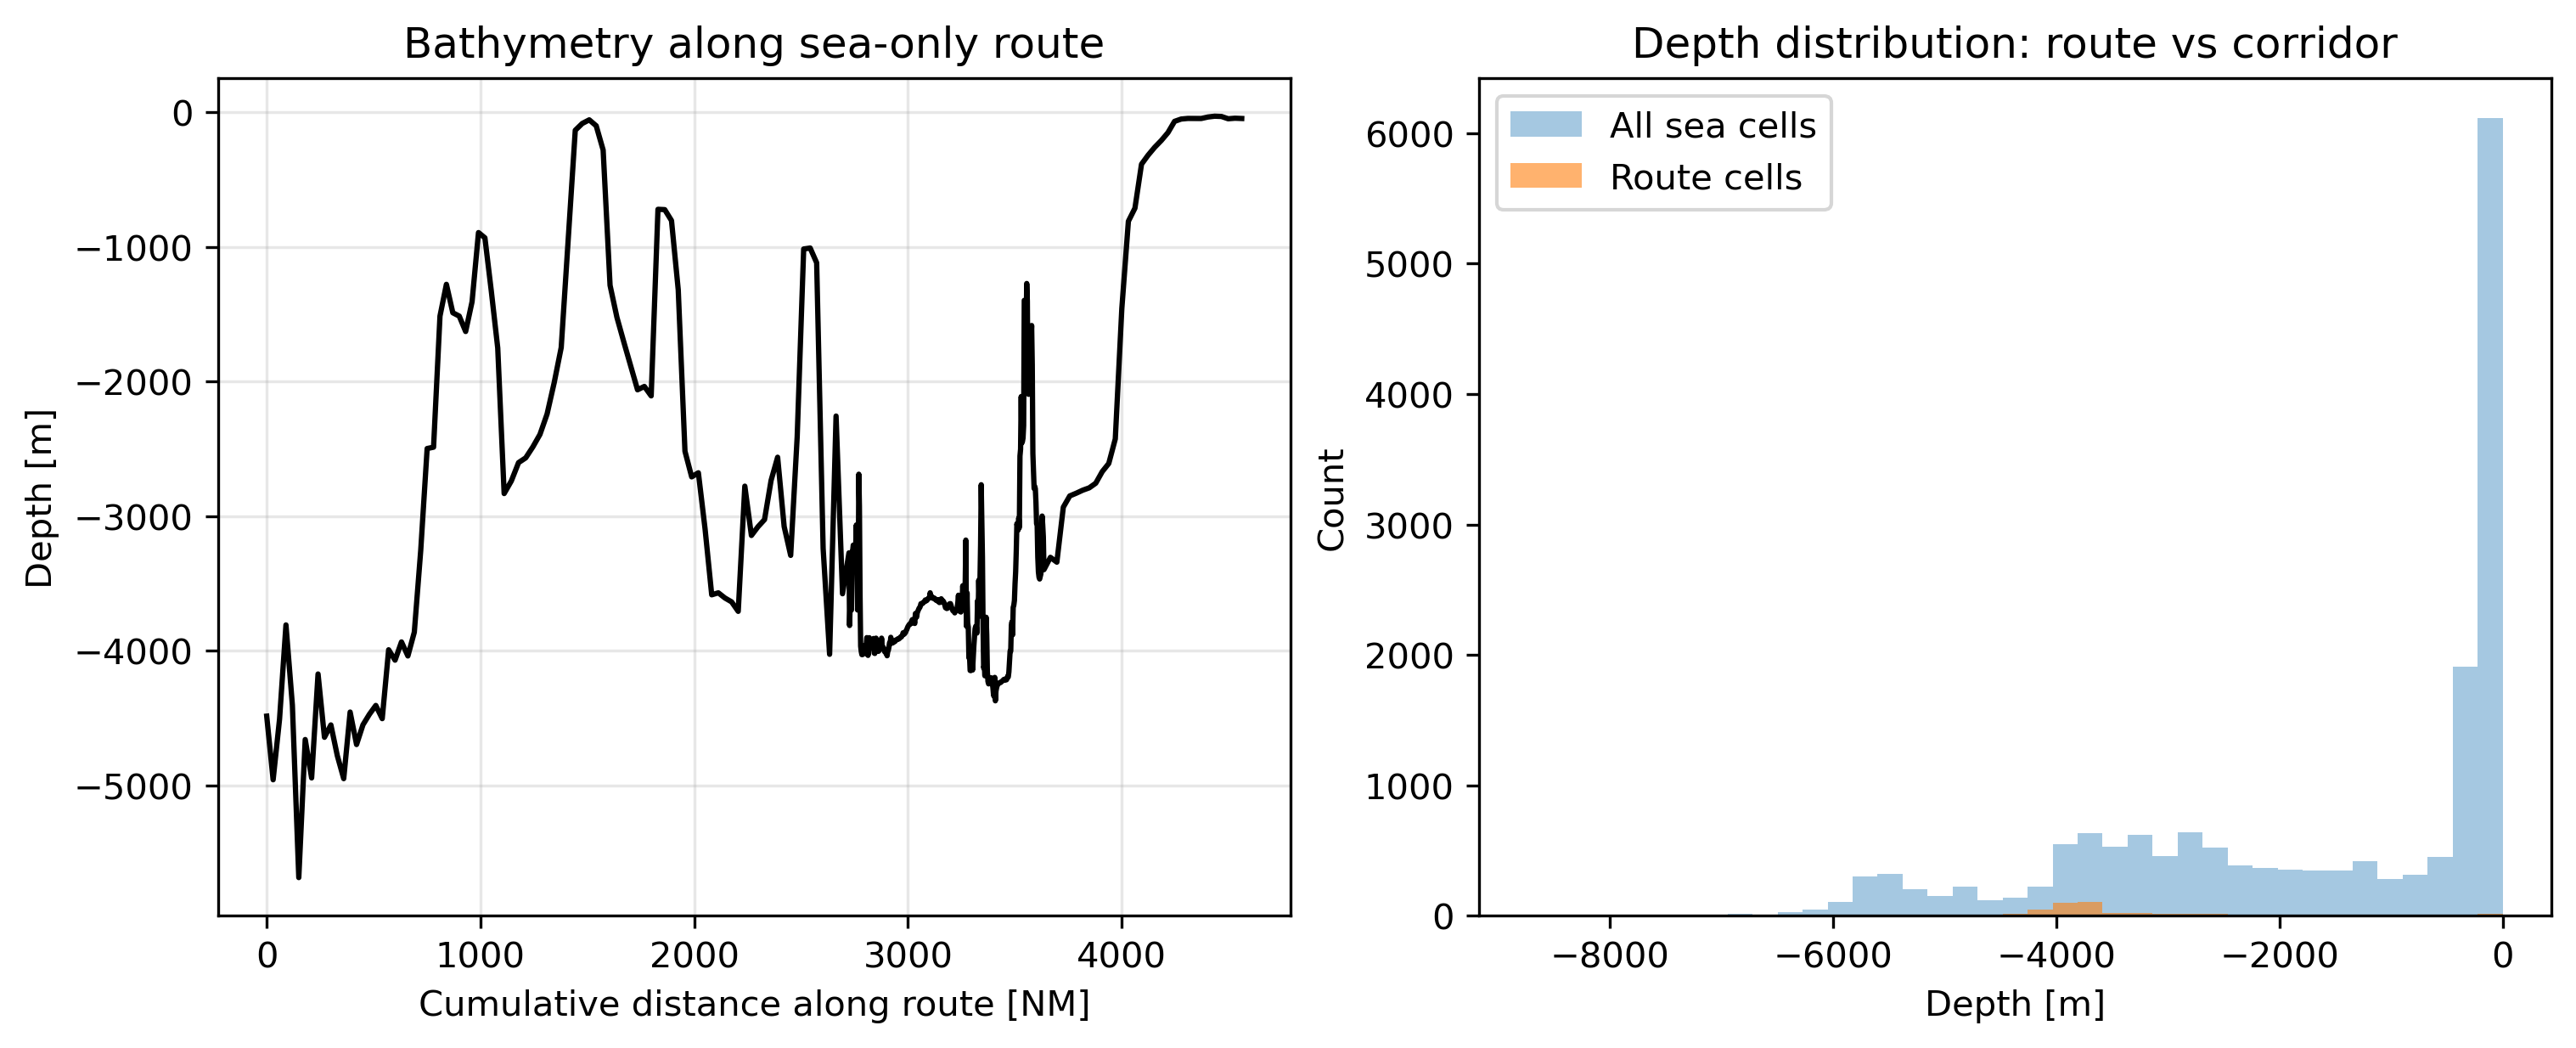
\includegraphics[width=\linewidth]{figS1_depth_along_route}
  \caption{%
  (a) Bathymetry along the baseline sea-only route as a function of cumulative
  distance. (b) Depth histograms for all sea cells in the corridor (blue) and
  for routed cells (orange); the route samples predominantly deep water and
  only briefly crosses shallow shelves.%
  }
  \label{fig:depth_profile}
\end{figure}


\subsection{Bathymetric safety thresholds and routing connectivity}
\label{sec:results_depth}

Having established a purely geometric sea-only route on the GEBCO-based grid,
we next examine how explicit bathymetric safety thresholds affect network
connectivity and route geometry. For a given minimum safe depth
\(h_\mathrm{min}\), the depth-safe sea mask \(M^\mathrm{depth}_{ij}(h_\mathrm{min})\) is
defined in Eq.~\eqref{eq:mdepth} as taking the value 1 where cell \((i,j)\) is
ocean and \(h_{ij} \le -h_\mathrm{min}\), and 0 otherwise; that is, only grid cells
deeper than \(h_\mathrm{min}\) are considered navigable.

In practice we apply this threshold to all interior cells of a candidate route,
while allowing the origin and destination cells themselves to be shallower
(``endpoints relaxed''), mimicking the fact that vessels typically enter or
leave deep-water routes through local port approaches.

On the $0.5^{\circ}$ routing grid, the static sea mask occupies
approximately $48\%$ of all cells. Imposing a relatively mild depth constraint
of $h_{\min}=20$~m retains $94\%$ of this sea area as depth-safe
($\approx 45\%$ of the whole grid) and leaves the canonical trans-Arctic
origin and destination in the same connected component. Running A* on this
depth-safe mask yields a route that is effectively identical to the baseline
sea-only path: the distance remains $4561$~NM, corresponding to a $10\%$
inflation over the great-circle distance, and depths sampled along the route
remain almost entirely in deep water
(Fig.~\ref{fig:depth_path_map}, cf.~Fig.~\ref{fig:depth_profile}). This confirms that, at the scale of our
corridor, the unconstrained sea-only route already follows the deep-ocean
backbone and does not exploit marginally shallow shortcuts.

As the minimum safe depth is tightened, the navigable network gradually
fragments. For $h_{\min}=50$~m, only about $85\%$ of the original sea area
remains depth-safe; by $h_{\min}=200$~m this drops to roughly two-thirds of the
sea mask. The number of depth-safe connected components increases from
$30$ to more than $35$ as the threshold is raised, and beyond
$h_{\min}\approx 50$~m the canonical origin and destination lie in different
depth-safe components (Fig.~\ref{fig:depth_connectivity}b). In other words, at
this resolution there is no continuous path between the Atlantic and Pacific
gateways that is everywhere deeper than 50--200~m.

The spatial pattern of these constraints is illustrated in
Fig.~\ref{fig:depth_path_map}a, where the sea-only route is overlaid on
bathymetry with selected isobaths. Narrow shallow features along the shelf
break and in straits appear as ``choke points'' that disconnect the deep-water
network once a stringent depth threshold is enforced. From an operational
perspective, vessels with realistic draughts could still transit these regions,
but at the $0.5^{\circ}$ grid spacing they collapse into single grid cells that
are either fully safe or fully blocked. This highlights an important trade-off:
coarser grids are computationally attractive for large-scale scenario analysis,
but they can overstate the impact of bathymetric constraints in narrow
passages.

A complementary diagnostic is provided by the depth distribution in the
corridor versus along the route
(Fig.~\ref{fig:depth_profile}). While the overall sea area spans depths from
approximately $-100$ to $-6000$~m, the A* route samples predominantly the
deeper part of this distribution, with a long tail towards abyssal depths and
only a small fraction of cells shallower than 100~m. Together with the
connectivity analysis, this suggests that in the present configuration
bathymetry is \emph{not} the primary limiting factor for a trans-Arctic
corridor at the coarse planning scale; rather, the static sea-only feasibility
and the seasonal sea-ice field (addressed in the following sections) are the
dominant controls on route availability.


\begin{figure}[htbp]
  \centering
  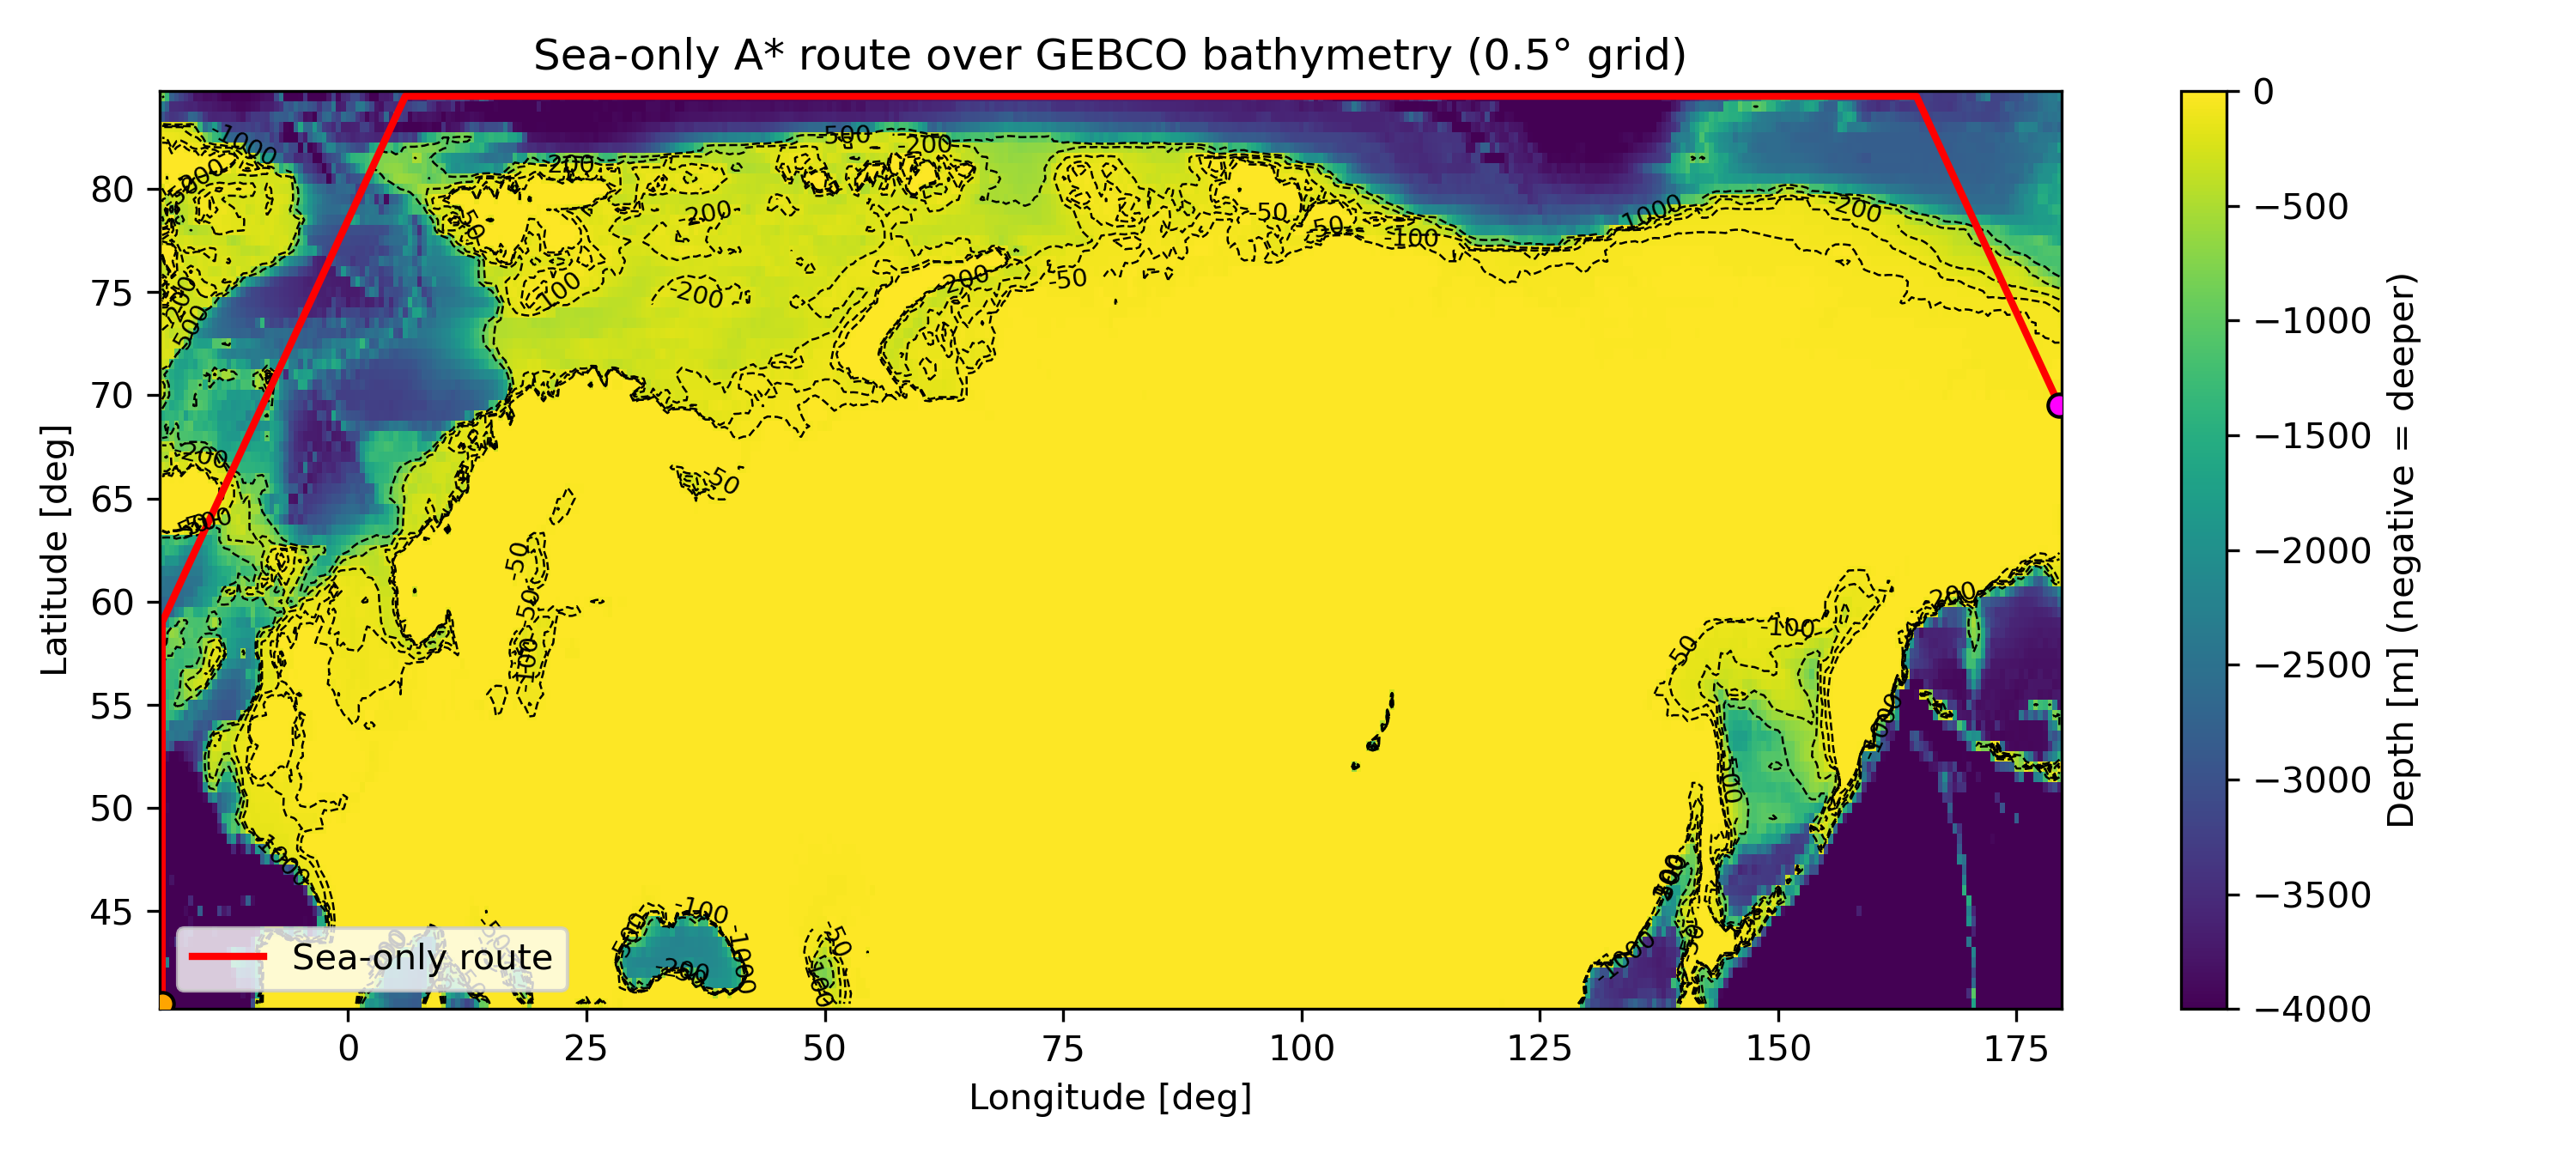
\includegraphics[width=\linewidth]{fig03_depth_path_map}
  \caption{%
  Sea-only A* route (red) over GEBCO~2024 bathymetry on the $0.5^{\circ}$ grid,
  with selected isobaths. The path tracks the Arctic shelf break and remains
  mostly in deep water even without explicit depth constraints.%
  }
  \label{fig:depth_path_map}
\end{figure}


\begin{figure}[htbp]
  \centering
  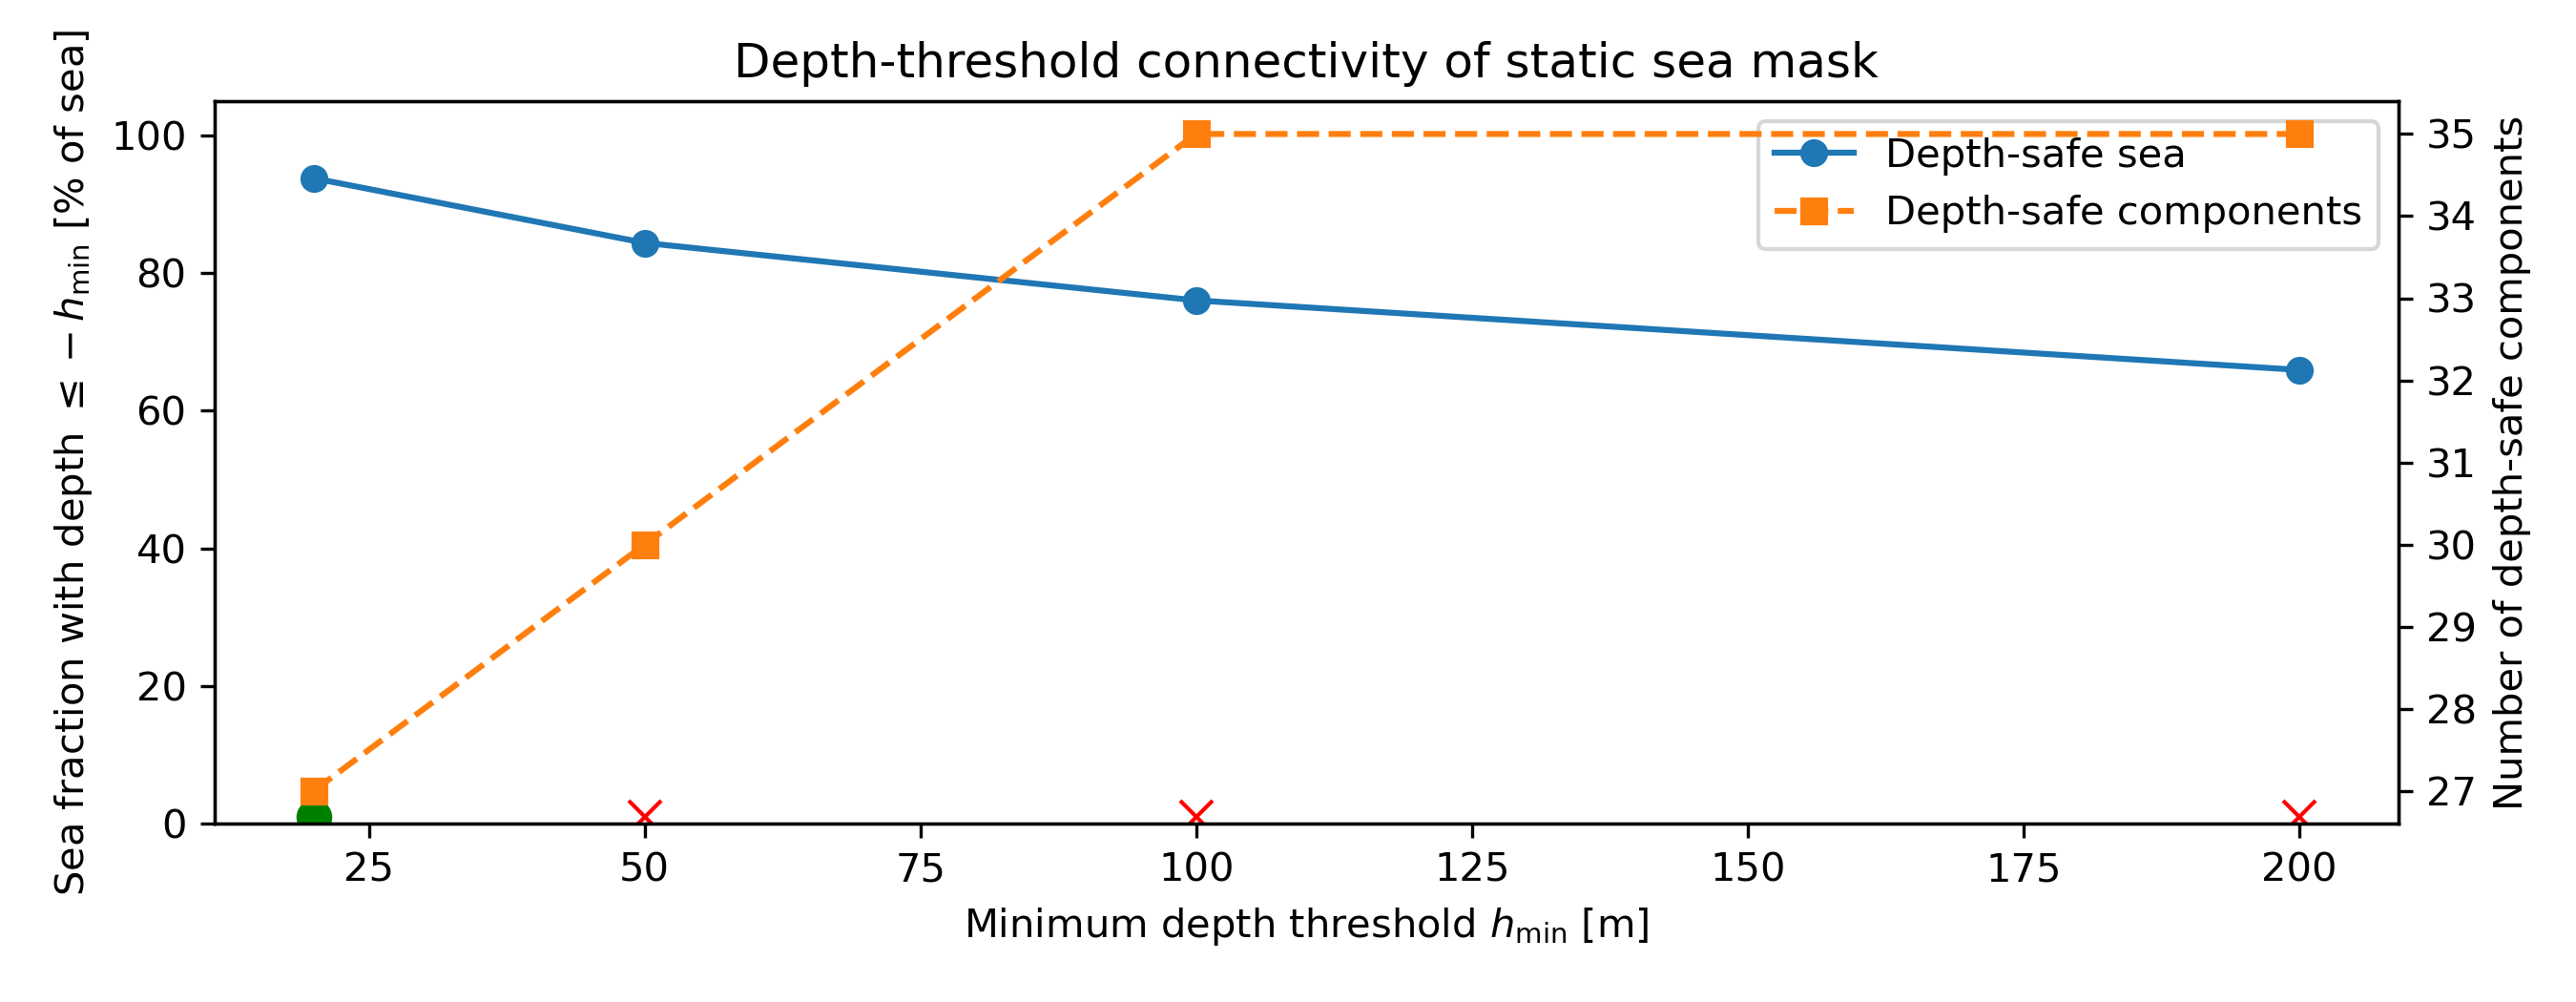
\includegraphics[width=0.9\linewidth]{fig04_depth_connectivity}
  \caption{%
  Effect of minimum depth $h_{\min}$ on the fraction of depth-safe sea area
  (blue, left axis) and the number of depth-safe components (orange, right
  axis). Markers indicate whether the canonical origin and destination lie in
  the same component (route possible) or not.%
  }
  \label{fig:depth_connectivity}
\end{figure}



\subsection{Seasonal opening of an ice-safe trans-Arctic corridor}
\label{sec:results_seasonal_ice}

We now investigate how seasonal sea-ice concentration modulates the feasibility
and geometry of the trans-Arctic corridor on the static bathymetric grid.
Sea-ice concentration (SIC) is taken from the CMEMS Arctic sea-ice reanalysis
for June--September 2018 and regridded onto the $0.5^{\circ}$ routing grid by
bilinear interpolation. For each target date we extract the nearest model time,
apply a fixed ice-safety criterion of $\mathrm{SIC}<15\%$, and intersect this
ice-safe mask with the static sea mask. The resulting ice-safe sea area and
associated connectivity are then evaluated for the canonical origin--destination
pair.

Figure~\ref{fig:seasonal_ice_area} shows the evolution of the ice-safe sea
fraction between mid-June and mid-September 2018, expressed as a percentage of
the static sea mask. In mid-June (15 June), only $58.6\%$ of the sea area is
ice-safe under the $\mathrm{SIC}<15\%$ criterion and the ice-safe domain is
fragmented into 96 disconnected components. By mid-July the ice-safe fraction
has increased to $65.5\%$ and the number of components has decreased to 66, but
no continuous ice-safe path exists between the Atlantic and Pacific gateways.
A qualitatively different regime emerges in late summer: by 15 August,
$77.0\%$ of the sea area is ice-safe and the number of components has dropped
to 33, at which point the canonical origin and destination first fall within
the same ice-safe component. By 15 September the ice-safe fraction reaches
$80.7\%$ of the static sea mask, still partitioned into 33 components, but with
a robust large-scale path spanning the Arctic.
These seasonal changes in ice-safe area, connectivity and route availability
are summarised in Table~\ref{tab:seasonal_ice_metrics}.

\begin{table}[htbp]
  \centering
  \caption{Seasonal evolution of ice-safe sea area and route availability for the
  canonical trans-Arctic origin--destination pair under the $\mathrm{SIC}<15\%$
  criterion. Ice-safe fractions are expressed relative to the static sea mask.
  ``Route'' indicates whether a continuous ice-safe path exists.}
  \label{tab:seasonal_ice_metrics}
  \resizebox{\linewidth}{!}{%
    \begin{tabular}{lccccc}
      \hline
      Date (2018) &
      Ice-safe sea [\% of sea] &
      Ice-safe components &
      Route &
      $D_{\mathrm{route}}$ [NM] &
      $\rho = D_{\mathrm{route}}/D_{\mathrm{GC}}$ \\
      \hline
      15 June      & 58.6 & 96 & No  & --     & --    \\
      15 July      & 65.5 & 66 & No  & --     & --    \\
      15 August    & 77.0 & 33 & Yes & 5206.0 & 1.255 \\
      15 September & 80.7 & 33 & Yes & 5019.9 & 1.210 \\
      \hline
    \end{tabular}%
  }
\end{table}

The impact of this seasonal evolution on routing is summarised in
Fig.~\ref{fig:seasonal_route_distance}. For the early-summer dates (15 June and
15 July) no ice-safe route exists under the $\mathrm{SIC}<15\%$ threshold, i.e.\
the trans-Arctic corridor is effectively \emph{closed} for the chosen
origin--destination pair despite the existence of a deep-water backbone. From
15 August onwards, an ice-safe sea-only route becomes available. On 15 August
its length is $5206$~NM, corresponding to a route-to-great-circle ratio of
$1.255$; by 15 September the distance has shortened to $5019.9$~NM and the
ratio to $1.210$. For comparison, the static bathymetry-based sea-only route
(ignoring ice) is $4561.1$~NM with a ratio of $1.099$ relative to the
$4149.6$~NM great-circle distance. Thus, even once the corridor is open in
late summer, the ice-safe route remains approximately $10\%$ longer than the
static sea-only path and about $20$--$25\%$ longer than the great-circle.

An illustrative late-summer ice-feasibility map and corresponding shortest
route are shown in Fig.~\ref{fig:ice_feas_map} for
15~September~2018. In mid-August, residual ice in the central Arctic and
along parts of the Siberian margin forces the route to skirt the ice edge,
yielding a strongly curved path that stays close to the deep
Norwegian--Greenland Sea and the Pacific side of the Arctic basin. By
mid-September, the ice extent has retreated further towards the central
Arctic and the marginal seas are largely accessible, allowing the route to
cut more directly across the basin and shorten by almost 200~NM. Despite
this shortening, the corridor remains substantially longer than both the
bathymetry-only path and the unconstrained great-circle.

Taken together, these results highlight that for a given bathymetric grid the
presence of sea ice imposes a \emph{binary} control on trans-Arctic feasibility
at seasonal timescales. For early-summer conditions in 2018 the chosen
origin--destination pair cannot be connected by any continuous ice-safe path
under a conservative $\mathrm{SIC}<15\%$ threshold, even though a deep-water
backbone exists. Once the corridor opens in late summer, sea-ice still adds a
second-order but non-negligible distance penalty on top of the static sea-only
inflation. This suggests that, from the perspective of large-scale voyage
planning, the timing of the seasonal ice retreat is a more critical driver of
trans-Arctic feasibility than moderate variations in the exact ice-safety
threshold, an aspect further explored in the threshold-sensitivity analysis in
Section~\ref{sec:results_ice_threshold}.



\begin{figure}[htbp]
  \centering
  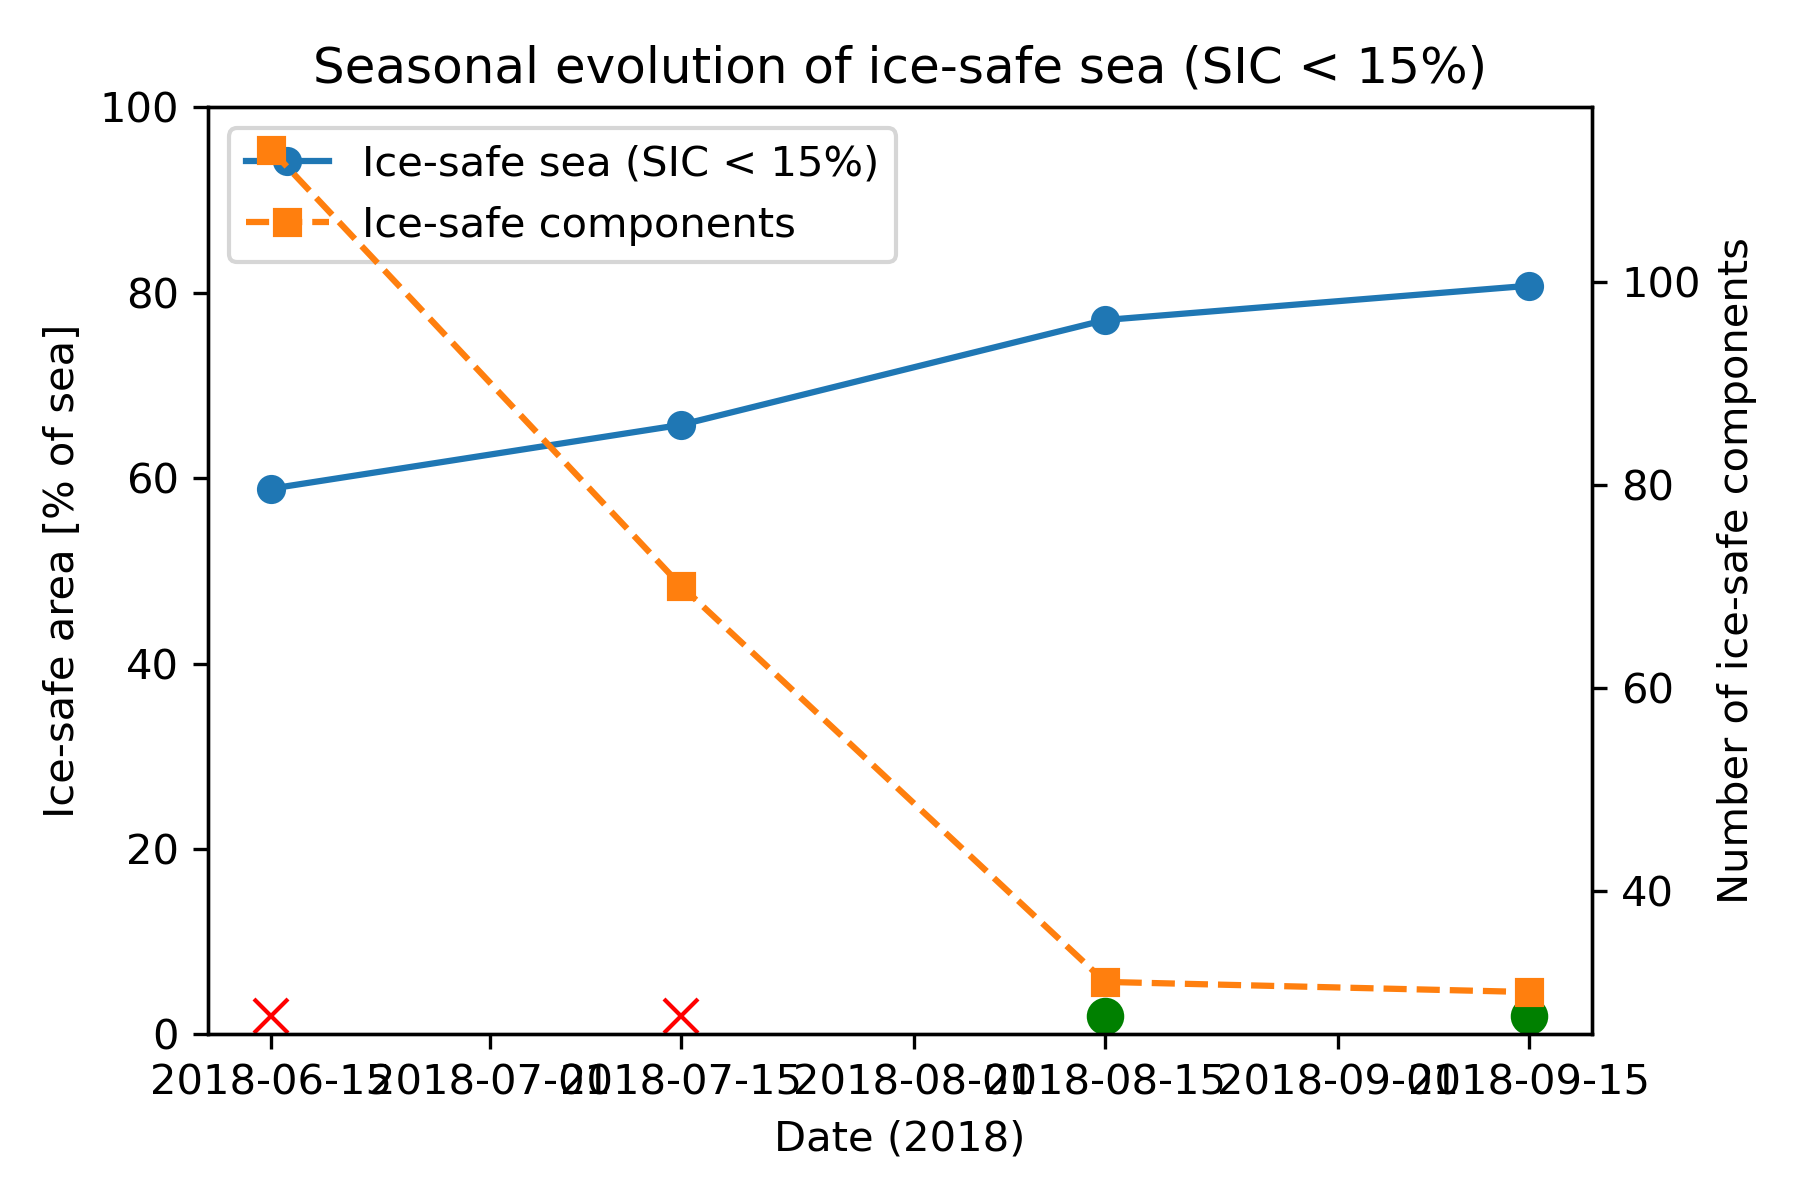
\includegraphics[width=0.9\linewidth]{fig05_seasonal_ice_area}
  \caption{%
  Seasonal evolution of the ice-safe sea fraction (blue, left axis) and number
  of ice-safe components (orange, right axis) for $\mathrm{SIC}<15\%$. Markers
  show dates when the canonical origin and destination lie in the same
  ice-safe component (route exists) or not.%
  }
  \label{fig:seasonal_ice_area}
\end{figure}



\begin{figure}[htbp]
  \centering
  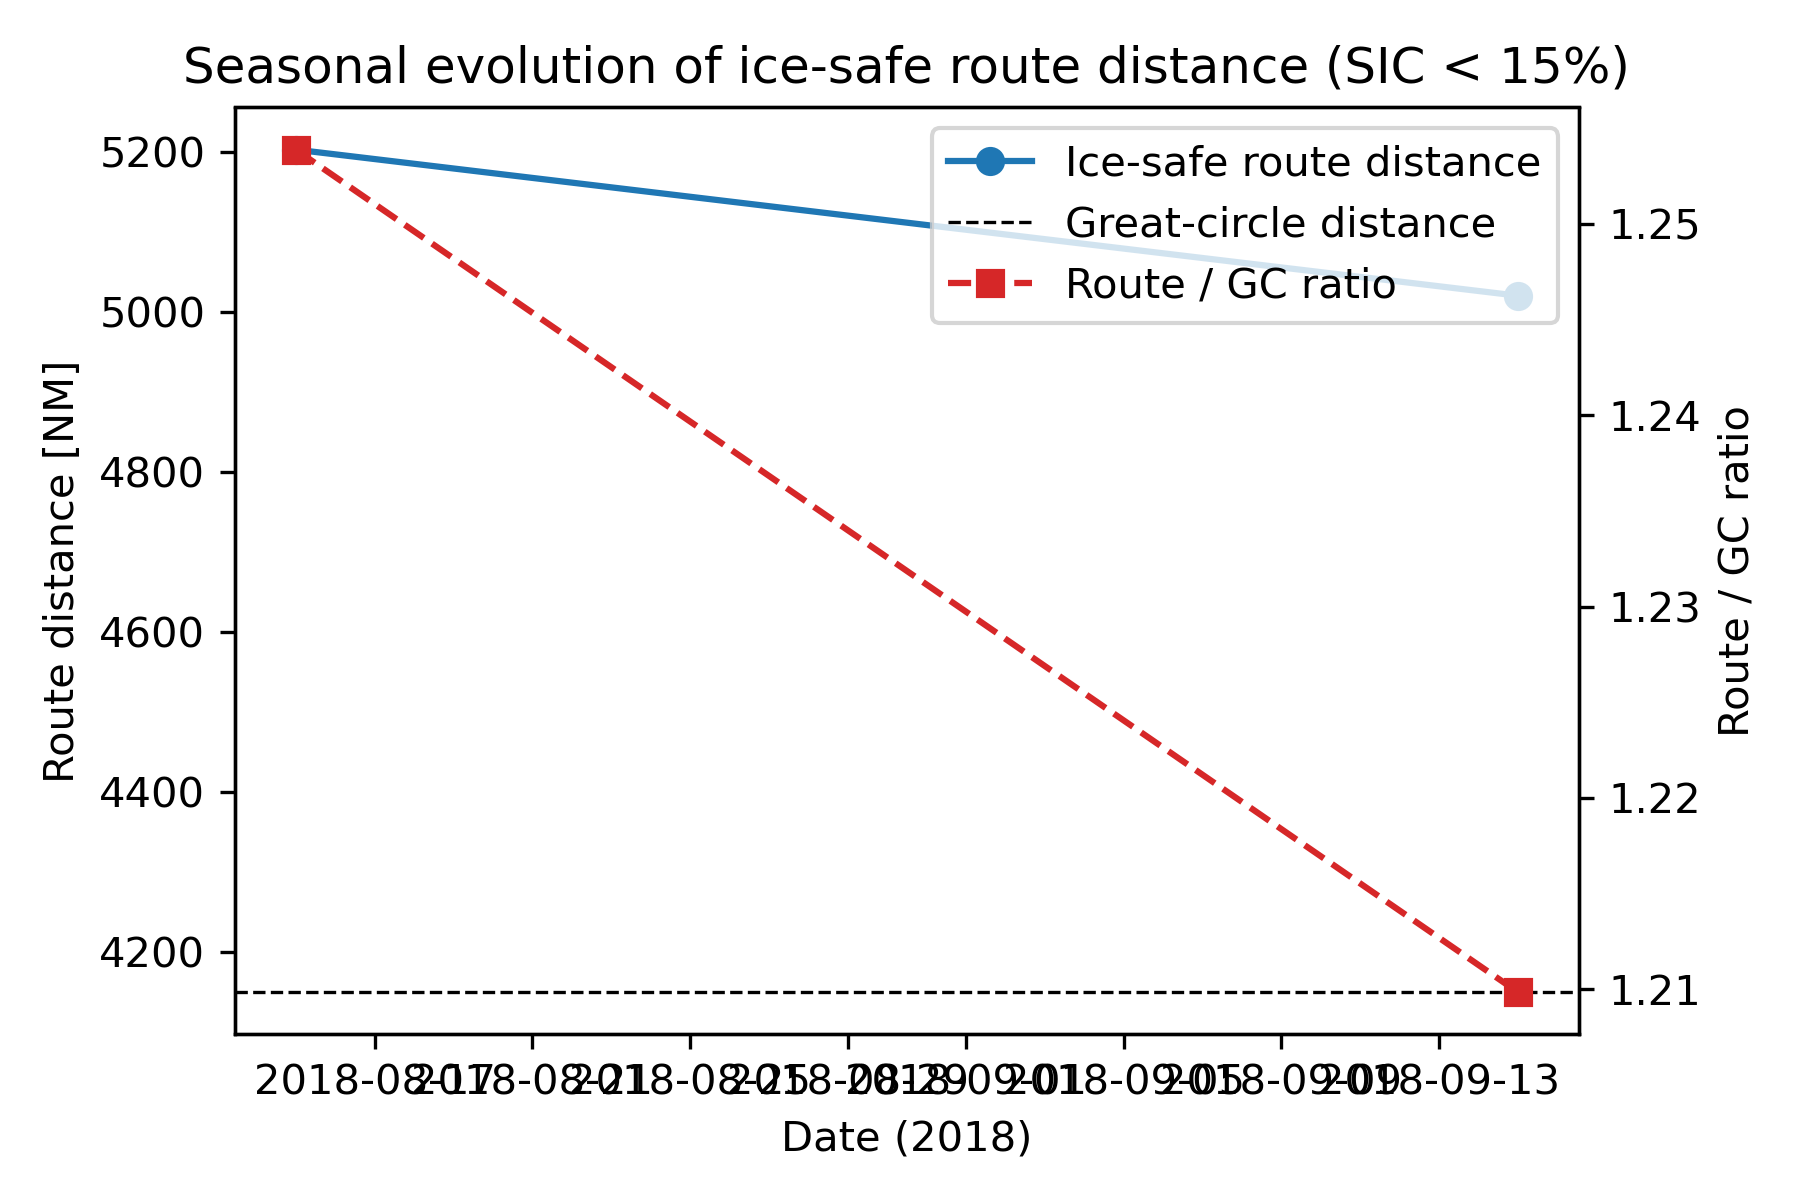
\includegraphics[width=0.9\linewidth]{fig06_seasonal_route_distance}
  \caption{%
  Seasonal evolution of the shortest ice-safe route distance (circles, left
  axis) and route-to-great-circle ratio (red dashed line, right axis) for
  $\mathrm{SIC}<15\%$. No route exists in June and mid-July; from mid-August
  the corridor opens and gradually shortens as ice retreats.%
  }
  \label{fig:seasonal_route_distance}
\end{figure}


\begin{figure}[htbp]
  \centering
  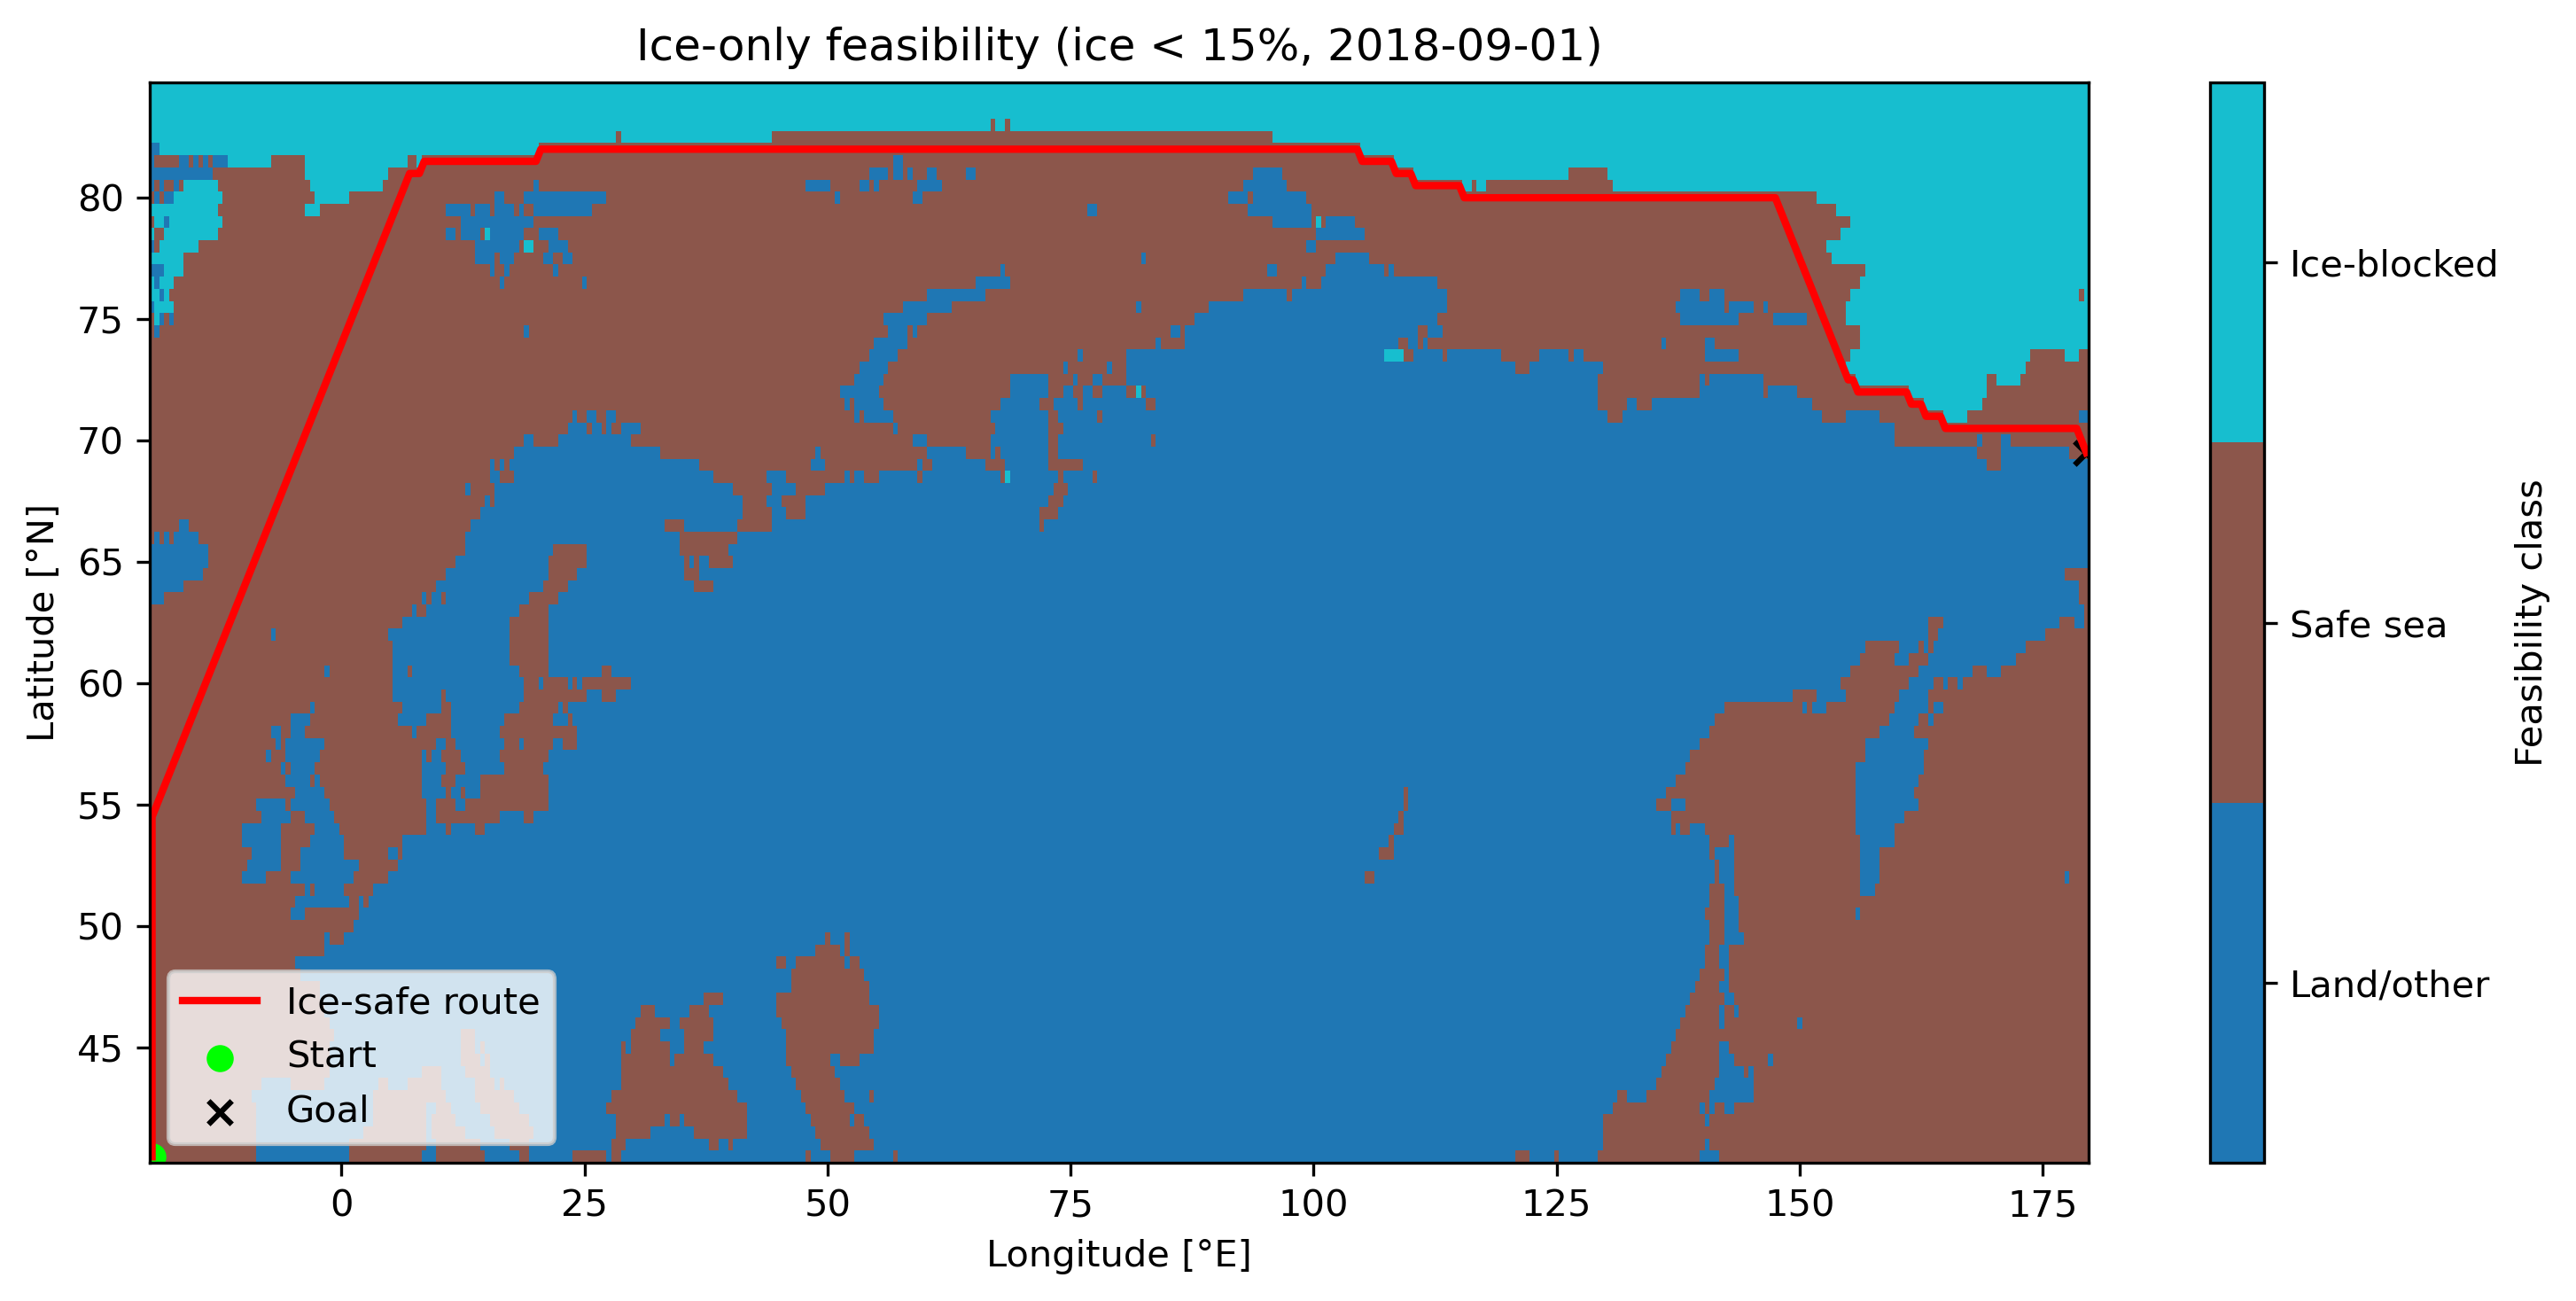
\includegraphics[width=\linewidth]{fig_ice_feasibility_20180901}
\caption{%
Ice-only feasibility on 15~September~2018 for the canonical origin--destination
pair under the $\mathrm{SIC}<15\%$ criterion. Brown shading shows ice-safe sea,
cyan shows sea blocked by ice, and blue indicates land or non-sea. The red line
is the shortest ice-safe route, with origin and destination marked.%
}
  \label{fig:ice_feas_map}
\end{figure}



\subsection{Sensitivity to the ice-safety threshold}
\label{sec:results_ice_threshold}

The previous section adopted a conservative but conventional ice-safety
criterion of $\mathrm{SIC}<15\%$ to define navigable sea. Here we examine how
sensitive the large-scale routing results are to this choice by varying the
threshold over a broad range of values and repeating the analysis.

We first fix the date to 15~September~2018, when the canonical
origin--destination pair is connected by an ice-safe route for the reference
threshold, and vary the ice-safety cut-off across $\mathrm{SIC}<5\%$, $10\%$,
$15\%$, $30\%$ and $50\%$. For each threshold we recompute the fraction of
static sea area that is ice-safe, the number of disconnected ice-safe
components, and, where possible, the shortest ice-safe A* route between the
Atlantic and Pacific gateways. As shown in
Fig.~\ref{fig:ice_threshold_curves}, the ice-safe area fraction increases only
modestly across this range, from approximately $80.4\%$ of the sea mask at
$\mathrm{SIC}<5\%$ to $81.5\%$ at $\mathrm{SIC}<50\%$. The number of
ice-safe components fluctuates between roughly 33 and 44, reflecting local
changes in the connectivity of marginal-ice zones, but the canonical origin
and destination remain in the same ice-safe component for all thresholds
considered.

The resulting route distances are remarkably insensitive to the choice of
threshold. For 15~September~2018, the shortest ice-safe sea-only path ranges
from $5024.5$~NM at $\mathrm{SIC}<5\%$ to $5018.6$~NM at
$\mathrm{SIC}<50\%$, corresponding to route-to-great-circle ratios between
$1.211$ and $1.209$. This spread of less than 6~NM and $<0.2\%$ in ratio is
negligible compared to the $\approx 10\%$ inflation relative to the
bathymetry-only sea route and the $\approx 20\%$ inflation relative to the
unconstrained great-circle distance. In other words, once the large-scale
trans-Arctic corridor is open, moderate tightening or relaxation of the
ice-safety threshold within the range 5--50\% has only a second-order effect on
route length.

To place this in a broader seasonal context, we extend the analysis to a grid
of dates and thresholds. For a set of representative dates between
15~June~2018 and 30~September~2018, and for each of the five thresholds, we
recompute the ice-safe mask and attempt to route the canonical
origin--destination pair. The resulting route-to-great-circle ratios are
summarised in Fig.~\ref{fig:heatmap_date_threshold_ratio}. Early in the
season (mid-June and early July), no continuous ice-safe path exists for any of
the thresholds in the 5--50\% range: the canonical gateways lie either outside
the ice-safe domain or in different disconnected components. The corridor thus
remains effectively closed, independently of the exact choice of
$\mathrm{SIC}$ cut-off.

A qualitatively different regime emerges once the seasonal ice cover retreats
sufficiently. From mid-August onwards, an ice-safe trans-Arctic route exists
for all tested thresholds, with route-to-great-circle ratios between
$\approx 1.25$ and $\approx 1.20$. The dominant gradient in the heatmap is
along the \emph{time} axis: ratios decrease from about $1.25$ in mid-August to
about $1.20$ by late September as the corridor widens and routes can cut more
directly across the basin. In contrast, variation along the threshold axis at a
given date is weak, typically at the level of a few tenths of a percent in
route length.

These results reinforce the interpretation that, at the scale of the present
corridor and grid, the seasonal timing of the ice retreat exerts a
first-order control on route feasibility and length, while the precise value
of the ice-safety threshold within a reasonable range primarily influences
local connectivity and the detailed shape of marginal-ice detours. For the
purposes of large-scale historical route diagnostics, a single reference
threshold such as $\mathrm{SIC}<15\%$ therefore appears adequate, provided
that the associated limitations for narrow passages and coastal approaches are
made explicit.

\begin{figure}[htbp]
  \centering
  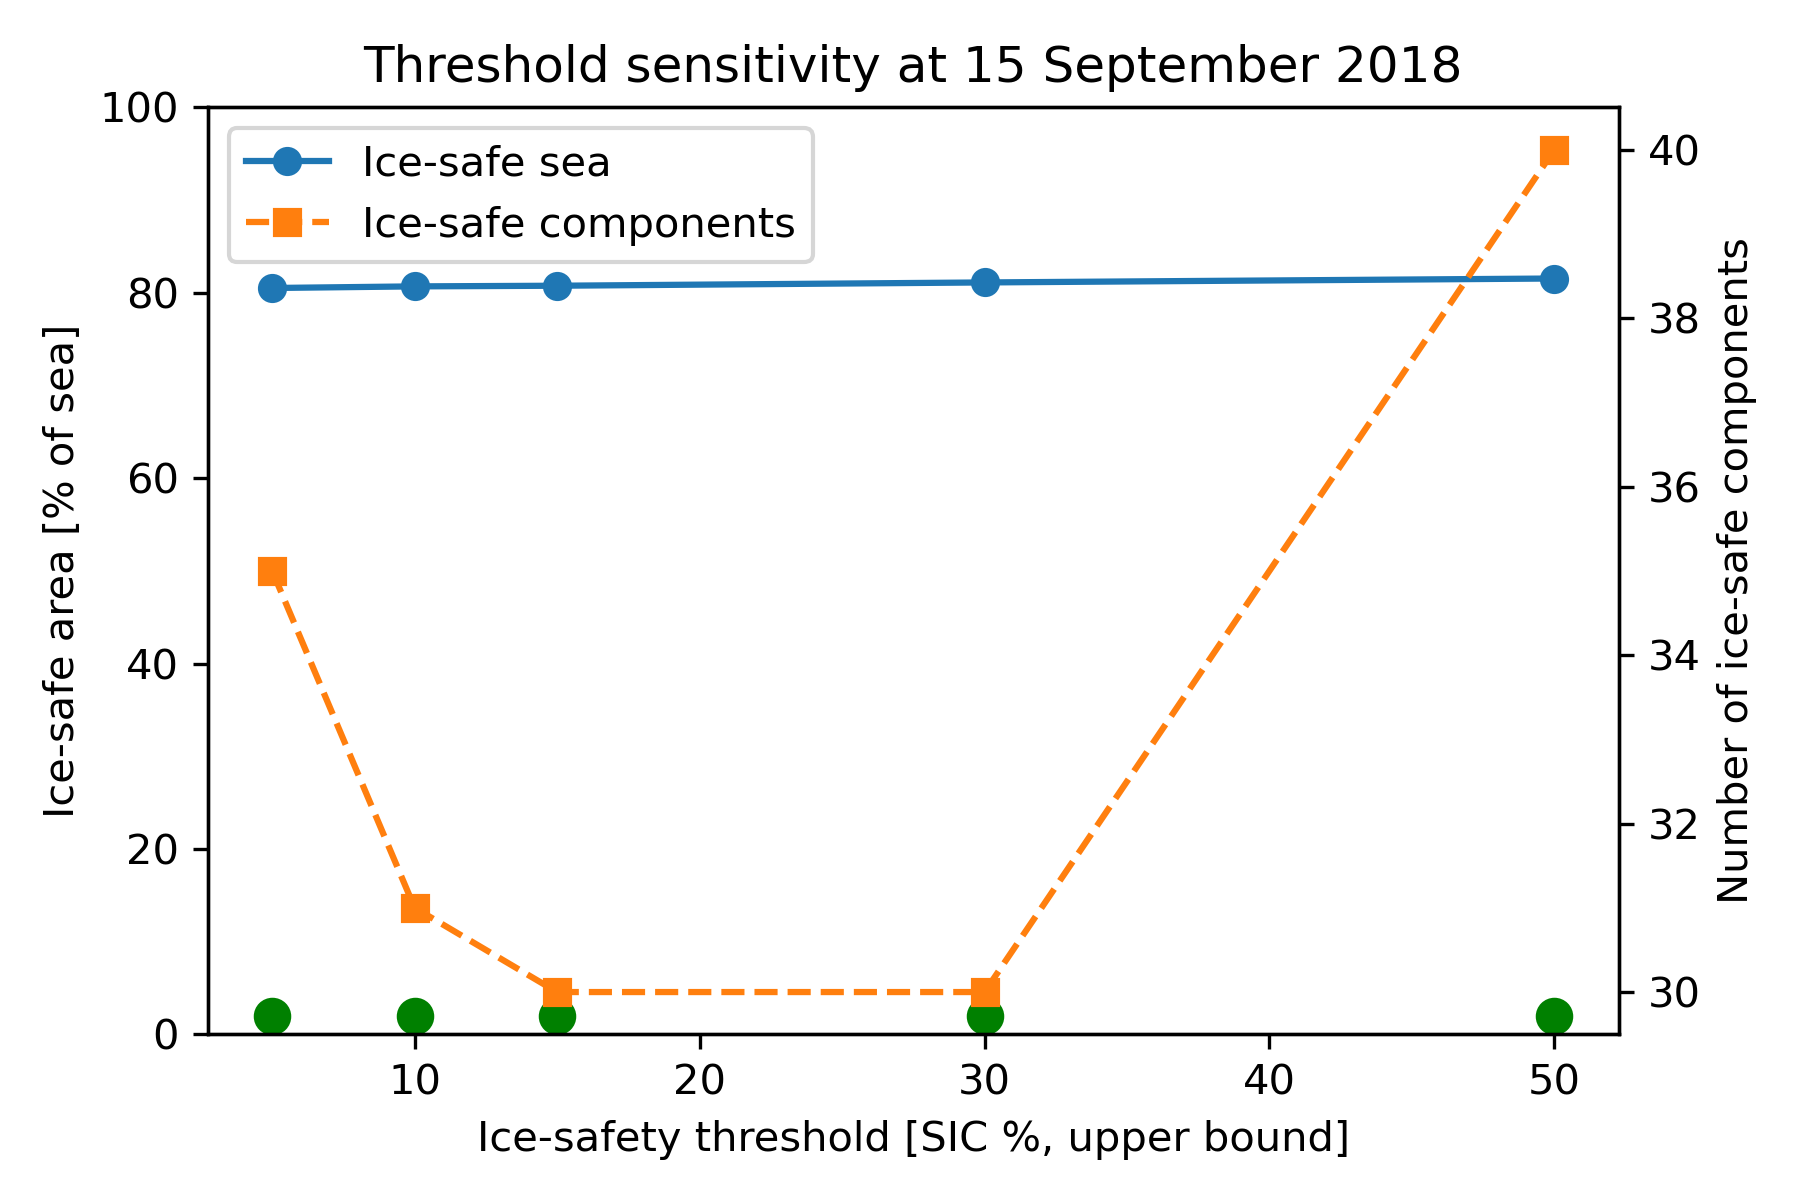
\includegraphics[width=0.9\linewidth]{fig07_ice_threshold_curves}
  \caption{%
  Sensitivity of ice-safe routing to the SIC threshold on 15~September~2018:
  fraction of ice-safe sea (blue, left axis), number of ice-safe components
  (orange, right axis), and OD connectivity (markers).%
  }
  \label{fig:ice_threshold_curves}
\end{figure}

\begin{figure}[htbp]
  \centering
  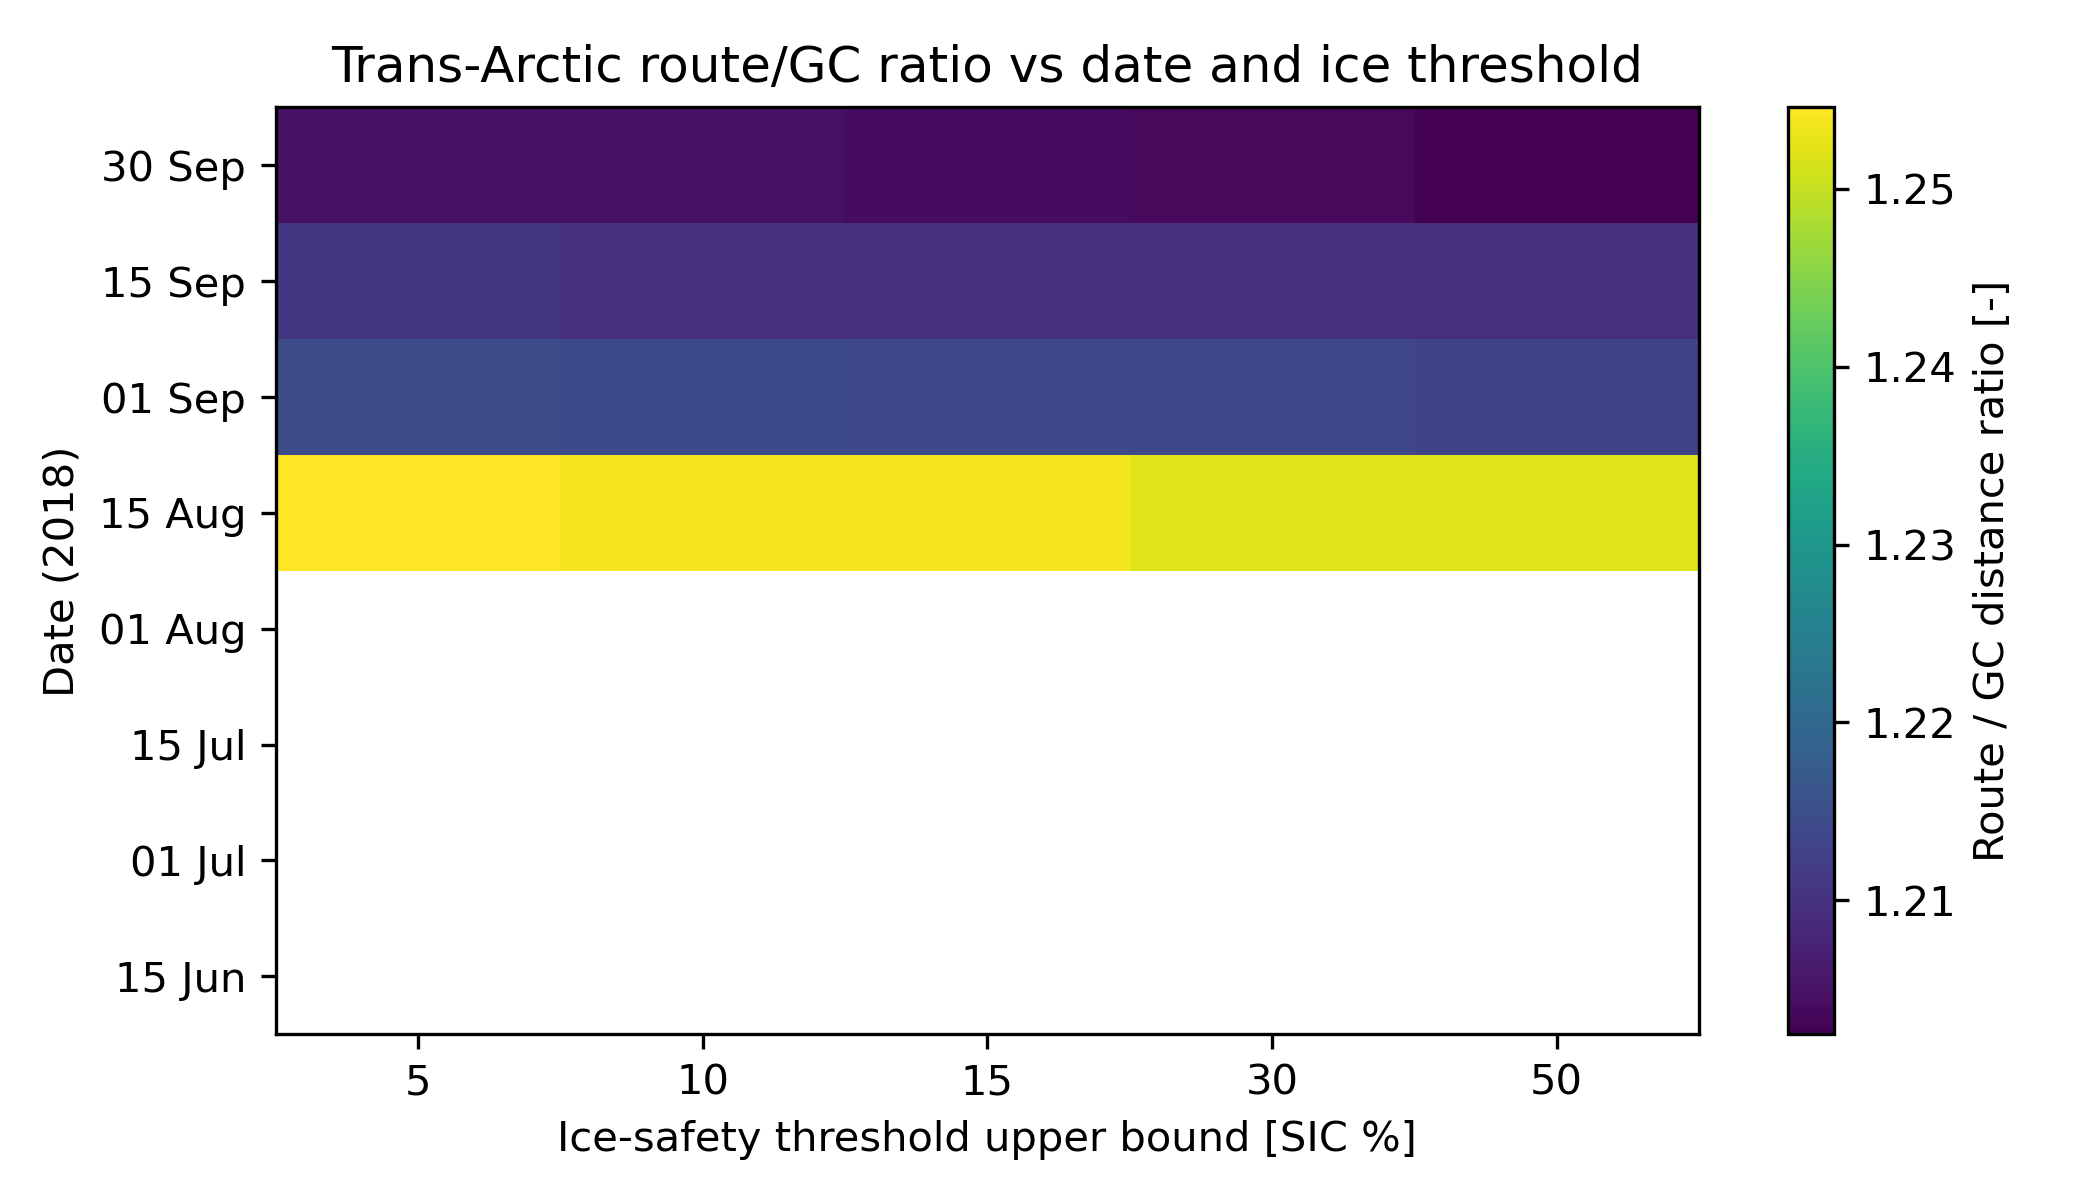
\includegraphics[width=\linewidth]{fig08_heatmap_date_threshold_ratio}
  \caption{%
  Route-to-great-circle distance ratio for the canonical origin--destination
  pair as a function of date and SIC threshold. Colours show ratios for the
  shortest ice-safe routes; white crosses indicate combinations with no
  continuous ice-safe path.%
  }
  \label{fig:heatmap_date_threshold_ratio}
\end{figure}


\subsubsection{Joint bathymetric and ice constraints}
\label{sec:results_joint}

The previous subsections considered bathymetric and ice constraints separately.
In a final diagnostic step we combined both into a joint feasibility mask,
requiring each routing cell to be (i) ocean, (ii) deeper than a minimum
under-keel clearance threshold $h_{\min}$, and (iii) ice-safe in the sense that
sea-ice concentration (SIC) remains below a navigational limit
$c_{\mathrm{ice}}^{\max}$.  Here we adopt $h_{\min}=20$~m and
$c_{\mathrm{ice}}^{\max}=15\%$ as representative values for unrestricted
open-water vessels and commonly used SIC thresholds in Arctic route screening.

For a late-summer snapshot (15~September~2018) the routing grid sea fraction
can be decomposed as follows.  Using only bathymetry, $93.8\%$ of the sea cells
are deeper than $20$~m, confirming that depth alone is not a primary limiting
factor at the $0.5^{\circ}$ corridor scale.  Using only ice, $80.8\%$ of sea
cells satisfy SIC~$<15\%$ on that date.  When both constraints are applied
simultaneously, the fraction of \emph{joint-safe} sea decreases to $74.6\%$ of
the sea mask.  While this reduction in area is modest, its spatial
organisation changes markedly: the joint-safe mask is split into
$35$ disconnected components on the $0.5^{\circ}$ grid.

Figure~\ref{fig:joint-depth-ice-mask} shows the resulting classification of the
Arctic corridor into land, sea blocked by either depth or ice, and joint-safe
sea.  The canonical trans-Arctic OD endpoints lie in different joint-safe
components (labels~1 and~20), so that no continuous route exists that
simultaneously respects $h_{\min}=20$~m and SIC~$<15\%$ along the entire path.
This is in stark contrast to the sea-only and ice-only experiments, where
late-summer Atlantic--Pacific connections could still be traced across the
same grid Table~\ref{tab:route_scenarios}. 

These results highlight that, even in a relatively favourable ice year such as
2018, the combination of shallow shelves and residual marginal ice is capable
of severing trans-Arctic connectivity at coarse resolution for realistic
under-keel and SIC thresholds.  In other words, large-scale
bathymetry-conditioned, ice-only route diagnostics (Sections~\ref{sec:results_depth}
and~\ref{sec:results_seasonal_ice}) are optimistic upper bounds on what can be
achieved when both constraints are enforced simultaneously.  From an
operational perspective this supports a two-step interpretation: (i) the
present paper’s sea-only and ice-only corridors provide an envelope of
\emph{where} and \emph{when} an Arctic route might be attractive at the basin
scale, while (ii) realistic planning for specific vessels and ports will
require higher-resolution bathymetry and sea-ice information, which we
address in subsequent work.


\begin{figure}[t]
  \centering
  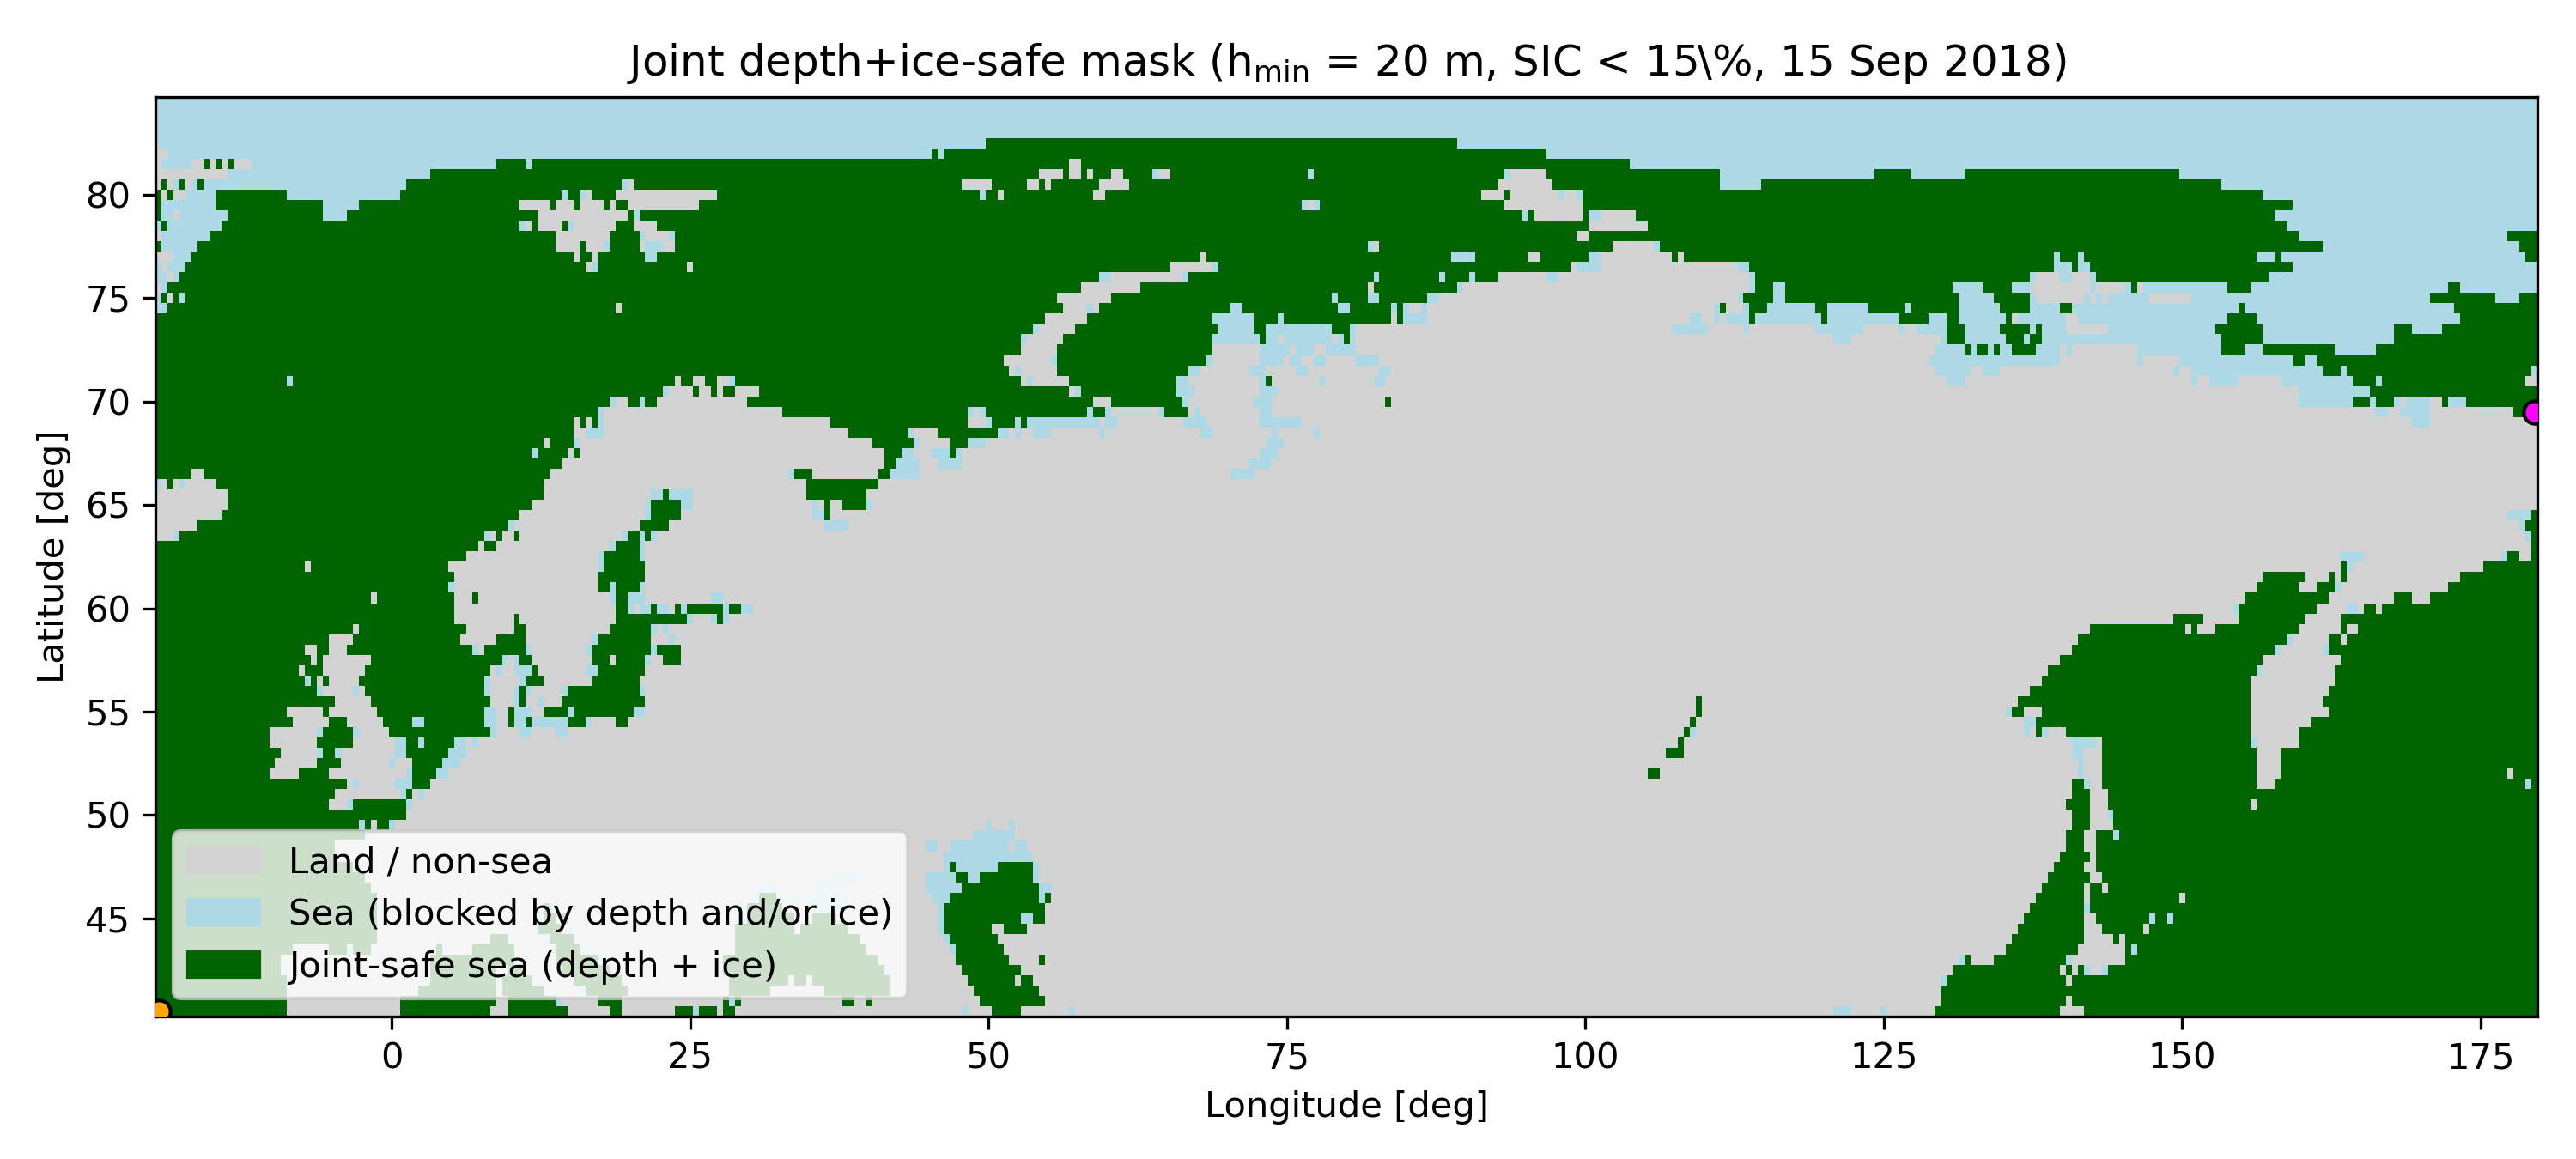
\includegraphics[width=\textwidth]{fig09_joint_depth_ice_mask}
  \caption{%
  Joint depth--ice feasibility mask ($h \ge 20$~m, SIC~$<15\%$) on the
  $0.5^{\circ}$ routing grid for 15~September~2018. Land, blocked sea and
  joint-safe sea are shown; the canonical origin and destination lie in
  different joint-safe components, so no continuous depth- and ice-safe route
  exists.%
  }
  \label{fig:joint-depth-ice-mask}
\end{figure}

\subsubsection{Summary of key implications for large-scale Arctic route diagnostics}
\label{sec:results-summary-implications}

The experiments in Sections~\ref{sec:results_bathy_baseline}–\ref{sec:results_joint}
allow a number of robust conclusions about large-scale Arctic route diagnostics on a
fixed geographic grid.
To provide context for these conclusions, Table~\ref{tab:route_scenarios}
summarises the canonical trans-Arctic route distance and inflation factor under
the main constraint combinations considered in this study.

\begin{table}[htbp]
  \centering
  \caption{Canonical trans-Arctic route distances and inflation factors under
  different constraint sets. $D_{\mathrm{GC}}$ is the great-circle distance
  between origin and destination; $D_{\mathrm{route}}$ is the A*-derived path
  length on the routing grid; $\rho = D_{\mathrm{route}}/D_{\mathrm{GC}}$.}
  \label{tab:route_scenarios}
  \resizebox{\linewidth}{!}{%
  \begin{tabular}{lccc}
    \hline
    Scenario &
    $D_{\mathrm{route}}$ [NM] &
    $\rho$ &
    Notes \\
    \hline
    Great-circle (unconstrained) &
    4149.6 & 1.000 &
    Theoretical lower bound \\
    Sea-only (GEBCO, static) &
    4561.1 & 1.099 &
    Land mask only; no ice or depth constraints \\
    Ice-only, 15 August 2018 ($\mathrm{SIC}<15\%$) &
    5206.0 & 1.255 &
    First date with continuous ice-safe corridor \\
    Ice-only, 15 September 2018 ($\mathrm{SIC}<15\%$) &
    5019.9 & 1.210 &
    Late-summer minimum of ice-constrained distance \\
    Joint depth+ice, 15 September 2018
    ($h_{\min}=20$~m, $\mathrm{SIC}<15\%$) &
    -- & -- &
    No continuous joint-safe route \\
    \hline
  \end{tabular}%
  }
\end{table}



First, enforcing sea-only feasibility on GEBCO~2024 already lengthens the canonical
trans-Arctic connection by about $10\%$ relative to a great-circle, even before
any environmental constraints are applied.  This confirms that widely used
rule-of-thumb shortcuts for trans-Arctic corridors underestimate path length once
sharp coastlines and islands are honoured on a realistic bathymetric grid.

Second, depth constraints at $0.5^{\circ}$ resolution are relatively benign for
open-ocean routing.  For representative under-keel limits of
$h_{\min}=20$--$50$~m, more than $85\%$ of the sea mask remains
depth-safe, and a sea-only route persists for $h_{\min}=20$~m.
Bathymetry therefore acts primarily as a static structural constraint, shaping
the corridor but not fundamentally blocking the basin-scale connection at this
resolution.

Third, historical sea-ice concentration is the dominant time-varying control on
trans-Arctic connectivity in the present framework.  The fraction of ice-safe
sea (SIC~$<15\%$) increases from roughly $60\%$ in mid-June to over $80\%$ in
mid-September, and a continuous trans-Arctic ice corridor only appears from
mid-August onwards.  Once open, the resulting ice-constrained routes are
systematically longer than the sea-only benchmark, but their excess distance
decreases by about 200 NM between August and late September as the
marginal ice zone retreats.

Fourth, at the large scales considered here the existence and length of an
ice-constrained route are only weakly sensitive to the exact SIC threshold in
the range $5$--$50\%$.  Changing the threshold modifies the fraction of
ice-safe sea by a few percentage points but only perturbs route length by
$\sim 20$–$30$~NM when a route exists.  For basin-scale diagnostics this suggests
that the choice of SIC threshold is less critical than the choice of season and
year, although it will matter more once finer grids and coastal passages are
resolved.

Finally, combining bathymetry and ice into a joint feasibility mask reveals that
even a relatively mild under-keel constraint ($h_{\min}=20$~m) can fragment the
apparently open late-summer ice corridor.  On 15~September~2018, only
$74.6\%$ of sea cells satisfy both depth and SIC criteria simultaneously, split
into $35$ disconnected components, and the canonical origin and destination fall
into different components.  At $0.5^{\circ}$ resolution there is therefore no
continuous route that is simultaneously sea-only, depth-safe and ice-safe along
its full length.

Taken together, these results position the present study as a basin-scale,
\emph{offline} screening tool: it quantifies how static bathymetry and
historical ice fields shape the feasibility and excess distance of trans-Arctic
routes, and delineates the temporal window during which such connections are
even theoretically possible.  In the companion work we build on this foundation
by moving to time-evolving forecasts, finer grids and multi-objective cost
functions better aligned with operational routing practice.